\documentclass[12pt]{report}
\usepackage[utf8]{inputenc}
\usepackage{graphicx}
\usepackage{float}
\usepackage[colorlinks=true, linkcolor=blue, urlcolor=blue, citecolor=black ]{hyperref}
\usepackage[spanish]{babel}
\usepackage{biblatex}
% TODOS: delete on finished document
\setlength {\marginparwidth }{2cm}
\usepackage{todonotes}
%
% \usepackage{xurl}
\usepackage{subfigure}
\addbibresource{references.bib}
\graphicspath{ {images/} }
% \setcounter{tocdepth}{3}

\title{
    {Desarrollo de videojuegos para un solo dev}\\
    {\large Universidad de Cuyo}\\
}
\author{Franco Sorbello}
\date{Day Month Year}

\begin{document}
\maketitle
\tableofcontents
% 
% ==== INTRODUCCIÓN ====
%
\chapter{Introducción}

\section{Motivación}

\par La industria de los videojuegos es destacada por su constante crecimiento y rentabilidad. No solo esto, si no que requiere una mano de obra altamente especializada. Programadores, músicos, artistas y escritores forman equipos para crear obras de arte interactivas. Sin embargo, la gestión de equipos tan diversos y la coordinación de múltiples tareas presenta un desafío considerable a la hora de llevar a cabo un proyecto de desarrollo de videojuegos.
\bigbreak
Este desafío aumenta al desarrollar un juego desde la perspectiva de un solo dev, es decir que el trabajo es llevado a cabo por una sola persona. El trabajo que comúnmente caería en otros miembros del equipo, como artistas o músicos, pasa a ser responsabilidad del desarrollador. Es por esto que este trabajo busca una metodología que permita llevar a cabo ese proceso de forma ágil y accesible.
\bigbreak
En general, en videojuegos no parece haber una línea clara a la hora de definir una metodología de trabajo. Por un lado, las metodologías ágiles, explicadas en el capítulo 2, parecen ser populares en el desarrollo de videojuegos. En 2013, Koutonen and Leppänen entrevistaron a 20 estudios finlandeses, donde todos menos uno indicaron que aplicaban Agile en al menos una de las fases de desarrollo \cite{koutonenHowAreAgile2013}.
En 2016, Politowski et al. entrevistaron a 58 desarrolladores brasileños y también encontraron un alto uso de metodologías ágiles \cite{politowskiSoftwareEngineeringProcesses2016}.
De forma similar, en 2021 McKenzie et al. entrevistaron a 8 estudios de Nueva Zelanda, los cuales indican utilizar alguna estrategia ágil, como Scrum o Kanban \cite{mckenzieAgileNotAgile2021}.
Finalmente, en 2025 Saarentaurus entrevistó a 5 productores de empresas de videojuegos finlandesas, y todos indicaron que utilizaban Agile en sus proyectos \cite{saarentausAgileScrumMethods2025}.
Estos productores trabajaban en empresas distintas, y todos tenían más de 5 años de experiencia en la industria. Cabe destacar que el estudio se realizó en empresas con más de 100 empleados \cite{saarentausAgileScrumMethods2025}.
\break
Si bien el tamaño de las muestras en cada estudio es pequeño, se puede notar que a lo largo de los años las metodologías ágiles han mantenido un nivel de relevancia en el desarrollo de videojuegos
\bigbreak
Otro fenómeno común al desarrollo es que los estudios terminen utilizando lo que se conoce como metodologías ad-hoc, que consiste en editar otros métodos de desarrollo con el objetivo de ajustarlas a las necesidades de la empresa. McKenzie et al. destacó que si bien los desarrolladores entrevistados indican usar metodologías ágiles, la mayoría realizan modificaciones a Scrum, como eliminar ciertas prácticas, o cambiar la duración de otras \cite{mckenzieAgileNotAgile2021}.
Estos cambios se deben a que es necesario adaptar Scrum a las particularidades del desarrollo de videojuegos \cite{mckenzieAgileNotAgile2021,bartoszScrumVideoGames2023}.
Como se explicó anteriormente, en la creación de un juego participan personas de áreas totalmente distintas, desde programación hasta música. Además, como los juegos son un producto de entretenimiento, uno de los requerimientos del software es que sea “divertido”. Esto es un problema a la hora de planificar ya que es difícil establecer objetivos basados en algo tan subjetivo como la diversión \cite{mckenzieAgileNotAgile2021,bartoszScrumVideoGames2023}. Es por esto que las empresas terminan realizando cambios a la metodología que adoptan.
\bigbreak
A esto se suma que algunos autores han propuesto metodologías específicas para el desarrollo de videojuegos. En 2024, Widjaja et al. desarrollaron un juego utilizando la metodología propuesta por Ramadan y Widyani \cite{widjajaUtilizingGameDevelopment2024}. Este sistema propone un modelo similar a modelos evolutivos pero incluye criterios de calidad relacionados con crear un producto “divertido” \cite{ramadanGameDevelopmentLife2013}. De forma similar, Harman propone un framework que separa distintas etapas del desarrollo en un método de cascada, y luego utiliza conceptos de metodologías ágiles en algunas de ellas \cite{harmanDevelopmentMethodologiesGame2023}.
\bigbreak
Hay un tercer grupo de desarrolladores que no es mencionado en los estudios anteriormente nombrados; los solo devs, o equipos pequeños (2-5 personas). La dinámica de desarrollo cambia debido a la poca cantidad de personas involucradas. No hay mucha investigación al respecto, pero de las fuentes obtenidas se puede observar el uso de metodologías ad-hoc, lo cual es congruente con lo mencionado anteriormente. Similar a Radaman, Widyani y Harman, Anderson separa el desarrollo en etapas de un método en cascada. Además, utiliza Kanban para organizar las tareas \cite{andersonProductionPointHow2023}. Robinson-Yu presenta una idea parecida, con el agregado de utilizar una versión simplificada de Scrum para llevar a cabo sus tareas \cite{gamedevelopersconferenceCraftingTinyOpen2020}.
\bigbreak
En este documento se estudian estas 3 vertientes, con el objetivo de formar una metodología que permita desarrollar un juego como solo dev, tomando los elementos que se consideren útiles y eliminando los que dificulten el trabajo.






\section{Objetivos}
El objetivo de este trabajo es encontrar un proceso de trabajo que permita desarrollar un videojuego como un solo dev. Para ello, se investigan herramientas y metodologías provenientes tanto del software tradicional como de los videojuegos.
\bigbreak
Los objetivos particulares derivados de lo anterior son:
\begin{enumerate}    
    \item Estudiar los frameworks utilizados en el software tradicional.
    \item Estudiar los frameworks específicos del desarrollo de videojuegos.
    \item Con la información anterior, crear un videojuego. Documentar el proceso, notando fortalezas y debilidades de la metodología elegida
\end{enumerate}






% 
% ==== ING DEL SOFTWARE ====
%
\chapter{Ingeniería de software}

\section{Definición de software}
En la actualidad, el software es una institución transversal al funcionamiento del mundo. Los gobiernos y otras entidades públicas son manejados mediante computadoras. Tanto el sector público como el privado utilizan la tecnología para automatizar la mayoría de industrias. Inclusive el arte es afectado por el software, con programas que asisten a la creación de música, pintura o video, entre otros \cite{sommervilleIngenieriaSoftware9a2011}.
\bigbreak
Formalmente, un software es definido como un “conjunto de programas de cómputo, procedimientos, reglas, documentación y datos asociados, que forman parte de las operaciones de un sistema de computación” \cite{alarconaldanaMetodologiaParaDesarrollo2020}. Sin embargo, el software tiene una serie de características que dificultan una definición única.
\begin{enumerate}
    \item El software se desarrolla o modifica con intelecto: los programas son productos intangibles, y por lo tanto no están regidos por procesos de fabricación comunes \cite{sommervilleIngenieriaSoftware9a2011,pressmanIngenieriaSoftwareEnfoque2013}
    \item El software no se desgasta: el software no es susceptible a las condiciones físicas que, por ejemplo, producen un desgaste en la usabilidad de un producto. Sin embargo, el software sí se deteriora. A lo largo de su desarrollo, el software sufre cambios que producen fallas. Estos cambios suelen traer mayor complejidad, por lo que estos errores aumenten en cantidad y dificultad \cite{sommervilleIngenieriaSoftware9a2011,pressmanIngenieriaSoftwareEnfoque2013}.
    \item El software se construye modularmente: a medida que una disciplina de la ingeniería avanza, se crean componentes estándar para utilizar en el diseño. Por ejemplo, tornillos, o circuitos integrados que están preconstruidos. Algo similar sucede en el software, donde se crean componentes reutilizables en otros programas, y sirven como ladrillos para construir nuevos programas \cite{sommervilleIngenieriaSoftware9a2011,pressmanIngenieriaSoftwareEnfoque2013}.
\end{enumerate}
\bigbreak
Por otro lado, a lo largo de los años han aparecido distintos tipos de software que satisfacen mercados variados. Se pueden encontrar:
\begin{itemize}
    \item \textbf{Software de sistemas}, que dan servicios a otros programas. Algunos ejemplos son compiladores, software de redes, o sistemas operativos \cite{pressmanIngenieriaSoftwareEnfoque2013}.
    \item \textbf{Aplicaciones independientes}, programas aislados que resuelven una necesidad específica y corren localmente en una PC \cite{sommervilleIngenieriaSoftware9a2011,pressmanIngenieriaSoftwareEnfoque2013}.
    \item \textbf{Software de ingeniería y ciencias}, que ayudan en procesos de investigación, simulación o cálculos matemáticos complejos.
    \item \textbf{Software embebido}, pensado para controlar dispositivos de hardware pequeños. Un ejemplo sería el panel de un microondas.
    \item \textbf{Aplicaciones web}, distinguidas por su fácil acceso, por lo general desde un navegador web.
    \item \textbf{Software de inteligencia artificial}, que utilizan algoritmos complejos para analizar grandes cantidades de datos.
\end{itemize}
\par
Esta tesina se enfoca en el videojuego, un arte nacido específicamente del software, y que no es capaz de existir fuera de él. Un aspecto interesante de ellos es que se ajustan a varios modelos. Pueden ser programas aislados, o tener conexión a servidores. En algunos casos, se pueden jugar desde un navegador web \cite{PhaserFastFun}. Inclusive, algunos motores gráficos se utilizan para simulación y entrenamiento de inteligencia artificial \cite{MLAgentsOverviewML,UnrealEngineAdvanced}.

\section{Etapas comunes} 
\par A medida que la tecnología avanza, el software se vuelve cada vez más complejo, con programas que requieren múltiples funcionalidades, integración con otros sistemas y constante cambio para ajustarse a las necesidades de los clientes.
\par Esta complejidad plantea desafíos a la hora de crear y mantener un software. Para abordar esta problemática, surgieron las metodologías de desarrollo de software (SDLC en inglés). El objetivo principal de las SDLC es simplificar el proceso de desarrollo y mantenimiento de software. Esto se logra mediante el uso de frameworks que definen una estructura clara para cada fase del ciclo de vida del software, desde la planificación inicial y el diseño, hasta la implementación, las pruebas, el despliegue y el mantenimiento a largo plazo \cite{sStudySoftwareDevelopment2017,rupareliaSoftwareDevelopmentLifecycle2010}. Generalmente, las SDLC comparten una serie de fases comunes a todos los frameworks.

\begin{enumerate}
    \item \textbf{Planning}: En esta etapa se comunica con el cliente y se establece la viabilidad y costo de desarrollar el software \cite{sStudySoftwareDevelopment2017,dwivediComparativeStudyVarious2022} . El objetivo es evaluar los objetivos de los participantes y reunir los requerimientos que ayuden a definir el producto final \cite{pressmanIngenieriaSoftwareEnfoque2013}
    \item \textbf{Definición de requerimientos}: En este paso se ahonda en las necesidades del cliente, mediante conversaciones y entrevistas con los consumidores y dueños del software. Luego, el equipo analiza cada requerimiento y evalúa las posibles ventajas y desventajas de llevarlo a cabo, además de las posibles dificultades técnicas y de diseño que traiga \cite{pressmanIngenieriaSoftwareEnfoque2013,sStudySoftwareDevelopment2017,dwivediComparativeStudyVarious2022}.
    \item \textbf{Diseño}: Las especificaciones del paso anterior se utilizan para plantear el diseño del software. El objetivo es crear un plan que guíe el desarrollo \cite{pressmanIngenieriaSoftwareEnfoque2013,sStudySoftwareDevelopment2017,dwivediComparativeStudyVarious2022}. En ciertas metodologías, este plan es final, e indica los objetivos a cumplir, los tiempos en los que se llevarán a cabo, y las entregas del software.
    \item \textbf{Desarrollo}: Como el nombre lo indica, esta etapa consiste en la creación de código y assets requeridos para el proyecto \cite{pressmanIngenieriaSoftwareEnfoque2013,sStudySoftwareDevelopment2017,dwivediComparativeStudyVarious2022}. Algunas herramientas comunes son lenguajes de programación como C\# o Javascript, además de debuggers\footnote{debugger:programa utilizado para detectar errores en un software.} y otras herramientas de testing \footnote{testing: proceso de detectar errores en un software.}.
    \item \textbf{Testing}: Se crea un ambiente de testing, donde los desarrolladores buscan errores en el software y sus distintas funcionalidades \cite{pressmanIngenieriaSoftwareEnfoque2013,sStudySoftwareDevelopment2017,dwivediComparativeStudyVarious2022}.
    \item \textbf{Deployment}: El software se vuelve accesible para los clientes. En algunos casos, se provee entrenamiento a los usuarios \cite{pressmanIngenieriaSoftwareEnfoque2013,sStudySoftwareDevelopment2017,dwivediComparativeStudyVarious2022}.
    \item \textbf{Mantenimiento}: Se continúa dando soporte al software a medida que es utilizado por los clientes \cite{pressmanIngenieriaSoftwareEnfoque2013,sStudySoftwareDevelopment2017,dwivediComparativeStudyVarious2022}.
\end{enumerate}


\section{Modelos lineales}
Los modelos lineales surgieron con el propósito de estructurar el desarrollo de software, que inicialmente carecía de orden. Constituyen la base de la ingeniería de software \cite{pressmanIngenieriaSoftwareEnfoque2013}. En ellos, el desarrollo se separa en etapas que se llevan a cabo de forma secuencial. Si bien en el presente se favorecen sistemas más interactivos, los modelos lineales son la base en la que se construye el desarrollo del software.
%
%
\subsection{Modelo en cascada}
\par El modelo en cascada es el más básico de las SDLC. En este modelo, se avanza por cada etapa secuencialmente, desde la concepción del producto hasta su entrega \cite{pressmanIngenieriaSoftwareEnfoque2013,sStudySoftwareDevelopment2017,dwivediComparativeStudyVarious2022}. Cada etapa es considerada un módulo independiente, y sólo se avanza cuando se ha completado \cite{dwivediComparativeStudyVarious2022}.
\par Durante la primera etapa, se establecen los requerimientos a completar, además de un plan de acción que engloba a todas las actividades de cada módulo. Cada fase genera uno o más documentos que permiten avanzar a la siguiente fase una vez que son aprobados \cite{sommervilleIngenieriaSoftware9a2011}. Este proceso se continúa hasta completar el software.
%
\begin{figure}[h]
  \centering
  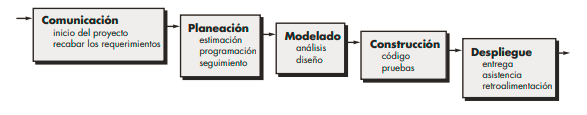
\includegraphics[scale=0.5]{image3.png}
  \caption{Modelo en cascada. Extraída de \cite{pressmanIngenieriaSoftwareEnfoque2013}.}
  \label{fig:x Modelo en cascada}
\end{figure}
%
\par Este modelo es el más antiguo de la ingeniería del software, ideado inicialmente en 1956 por el autor Herbert Bennington y luego modificado por Winston Royce en 1970 [17].
El modelo original, provisto por Bennington, recomendaba desarrollar el software en etapas separadas. Royce luego reconoció que en situaciones reales podrían aparecer dificultades inesperadas, por lo que su versión de cascada añade puntos de retorno en cada etapa, en caso de que sea necesario revisitar un estado anterior \cite{rupareliaSoftwareDevelopmentLifecycle2010,royceManagingDevelopmentLarge1970}. Sin embargo, la mayoría de las organizaciones aplican este modelo de forma estrictamente lineal \cite{pressmanIngenieriaSoftwareEnfoque2013}.
\begin{figure}[h]
  \centering
  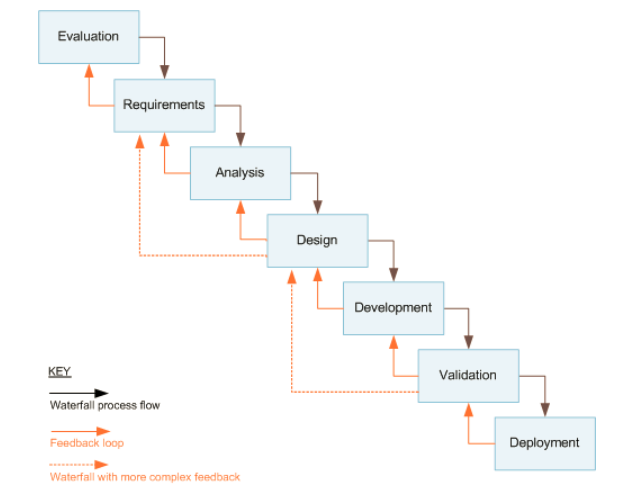
\includegraphics[scale=0.5]{image2.png}
  \caption{Modelo en cascada propuesto por Bennington. Extraída de \cite{rupareliaSoftwareDevelopmentLifecycle2010}.}
  \label{fig:x Modelo en cascada propuesto por Bennington}
\end{figure}
\subsubsection{Ventajas}
\begin{itemize}
  \item Útil para proyectos pequeños donde haya fases claramente definidas.
  \item Cada fase genera un producto entregable.
  \item Documentación extensa de los procesos y resultados.
\end{itemize}
\subsubsection{Desventajas}
\begin{itemize}
  \item Mucha resistencia al cambio, hace que sea difícil implementar en situaciones reales donde los requisitos varían constantemente.
  \item Los requerimientos se establecen al principio y no se pueden cambiar.
  \item No se obtiene un producto funcional hasta el final del proceso.
\end{itemize}
%
%
\subsection{Modelo en V}
\par El modelo en V, también conocido como el modelo de validación y verificación, es una variación del modelo en cascada \cite{rupareliaSoftwareDevelopmentLifecycle2010} donde se añade una segunda lista de etapas en dirección contraria, que retorna feedback para cada uno de los módulos llevados a cabo durante el desarrollo \cite{pressmanIngenieriaSoftwareEnfoque2013,rupareliaSoftwareDevelopmentLifecycle2010,dwivediComparativeStudyVarious2022}.
%
\begin{figure}[h]
  \centering
  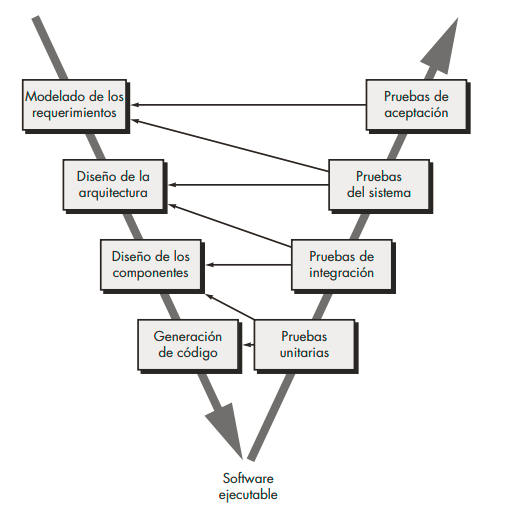
\includegraphics[scale=0.5]{image7.png}
  \caption{Modelo en cascada V. Extraída de \cite{pressmanIngenieriaSoftwareEnfoque2013}.}
  \label{fig:x modelo en v}
\end{figure}
%
\subsubsection{Ventajas}
\begin{itemize}
    \item Se adapta bien en proyectos con requerimientos claramente definidos.
    \item El proceso de validación genera un producto robusto.
\end{itemize}
\subsubsection{Desventajas}
\begin{itemize}
    \item Al igual que el método en cascada, es muy resistente al cambio de requerimientos.
    \item El proceso de validación no se realiza hasta que el software esté completado.
\end{itemize}

\section{Modelos incrementales}
\par En ciertos proyectos, el alcance del software es muy grande para desarrollarse de forma lineal. También puede suceder que es necesario entregar un software funcional en un corto plazo \cite{pressmanIngenieriaSoftwareEnfoque2013}. Para estos casos se pueden utilizar los modelos incrementales.
\par En este tipo de modelos, el software se avanza a partir de entregas incrementales, donde cada incremento suma nuevas funcionalidades. Generalmente, las primeras entregas incluyen los requerimientos urgentes, de forma que el cliente pueda validarlos en una etapa temprana del desarrollo \cite{sommervilleIngenieriaSoftware9a2011,pressmanIngenieriaSoftwareEnfoque2013}.
\par Cada uno de estos incrementos sigue el ciclo de vida en cascada, es decir que el desarrollo de una iteración se separa en módulos que deben ser terminados para avanzar al siguiente \cite{gujarathiSpiralDevelopmentNonSoftware2024}.
%
\begin{figure}[h]
  \centering
  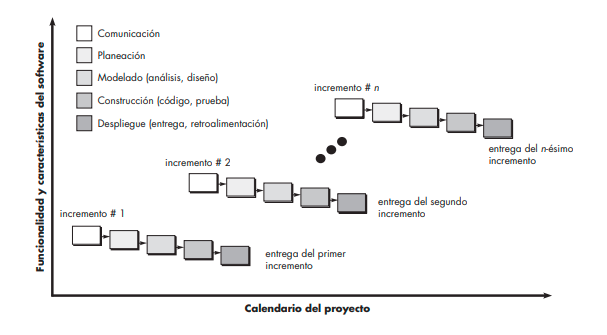
\includegraphics[scale=0.8]{image5.png}
  \caption{Modelo incremental . Extraída de \cite{pressmanIngenieriaSoftwareEnfoque2013}.}
  \label{fig:x Modelo incremental}
\end{figure}
\par El desarrollo incremental es particularmente útil cuando no se dispone del personal para la implementación completa del producto. Un equipo pequeño puede crear una versión básica del proyecto, y escalar a medida que la empresa crece \cite{pressmanIngenieriaSoftwareEnfoque2013}. 
Sin embargo, ciertas desventajas aparecen con este tipo de metodologías. En un principio, es difícil medir el progreso de un proyecto cuando las entregas se crean en rápida sucesión. A esto se suma que la estructura del sistema tiende a degradarse con el paso del tiempo debido a la periodicidad de cambios \cite{sommervilleIngenieriaSoftware9a2011}.


\section{Modelos evolutivos}
\label{sec:modelos_evolutivos}
\par El software evoluciona con el tiempo. Los requerimientos de negocio y producto se modifican conforme avanza el desarrollo, y los constantes cambios en el mercado hacen que sea muy difícil desarrollar un software en tiempo y forma. Para esto existen los modelos evolutivos, que están diseñados explícitamente para adaptarse a un producto evoluciona con el tiempo \cite{pressmanIngenieriaSoftwareEnfoque2013}. Los modelos evolutivos son iterativos. Están pensados para desarrollar versiones cada vez más completas del software
%
%
\subsection{Modelo en espiral}
\par El modelo en espiral se acopla la naturaleza iterativa de hacer prototipos con el aspecto más lineal y controlado de los métodos en cascada. El software se desarrolla en una serie de entregas evolutivas, donde en cada iteración se obtiene una versión más completa del software \cite{pressmanIngenieriaSoftwareEnfoque2013}.
\begin{figure}[H]
  \centering
  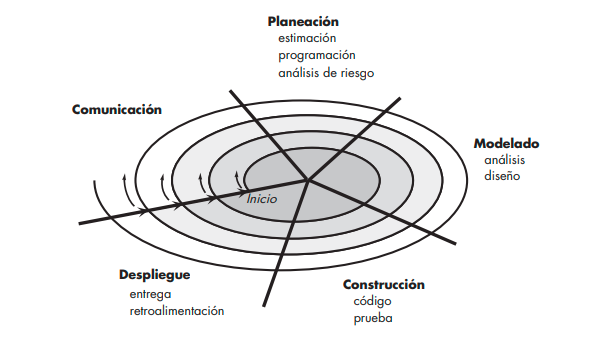
\includegraphics[scale=0.8]{image10.png}
  \caption{Modelo en espiral. Extraída de \cite{pressmanIngenieriaSoftwareEnfoque2013}.}
  \label{fig:x Modelo en espiral}
\end{figure}
\par El modelo en espiral se divide en un conjunto de actividades estructurales que se repiten en cada iteración. El primer circuito resulta en la especificación del producto. Las vueltas sucesivas se usan para desarrollar el prototipo y finalmente el resto de iteraciones son para crear el producto final \cite{pressmanIngenieriaSoftwareEnfoque2013}.

\section{Metodologías ágiles}
\par Las metodologías ágiles aparecen por la necesidad de una metodología flexible y capaz de adaptarse a los constantes cambios \cite{bartoszScrumVideoGames2023}. Estas metodologías se desarrollan en los años 90, y nacen de la frustración que las empresas percibían respecto a metodologías lineales \cite{sommervilleIngenieriaSoftware9a2011,pressmanIngenieriaSoftwareEnfoque2013}. 
El objetivo es que el equipo de desarrollo se enfoque en crear el software en vez de diseñar y documentar. Además, toman conceptos del desarrollo incremental, donde el producto se avanza generando iteraciones que son entregables a un cliente \cite{pressmanIngenieriaSoftwareEnfoque2013}.

\par Hay varias implementaciones de metodologías ágiles. Una de las más populares es Scrum, explicada en la sección a continuación.

\section{Scrum}
\par Tango Scrum como el resto de metodologías ágiles nacen de la necesidad de una metodología flexible y adaptable a los constantes cambios de los mercados tecnológicos \cite{bartoszScrumVideoGames2023}. Es una respuesta a las metodologías tradicionales, como Waterfall, las cuales priorizan seguir un plan definido \cite{cynthiachizobaekechiEnhancingAgileProduct2024}. En este sentido, Scrum representa un cambio de paradigma, que se enfoca en un sistema flexible, iterativo y colaborativo sobre el acercamiento basado en planes estrictos y documentación.
\par Scrum se basa en la idea de dividir el desarrollo de un software en pequeñas iteraciones llamadas sprints, generalmente durando un máximo de 4 semanas. El objetivo es que cada sprint produzca incrementalmente un producto usable, el cual puede ser presentado a un usuario final \cite{bartoszScrumVideoGames2023}.
\par Hoy en día, las empresas trabajan para crear productos digitales que satisfagan las necesidades de sus clientes, no sólo en videojuegos, si no que en la industria del software en general. Esto presenta un mayor desafío para una empresa pequeña, que aún debe competir en un mercado global a pesar de tener menos recursos \cite{putrianasariProblemsAdoptionAgileScrum2024}.Es por esto que muchas empresas implementan Scrum, una metodología que acepta el cambio constante y prepara a la institución para un ambiente dinámico y un futuro incierto \cite{putrianasariProblemsAdoptionAgileScrum2024}.
\par Scrum se basa en una serie de principios, donde los principales son:
\begin{itemize}
  \item Equipos autogestionados: a diferencia de otras metodologías, que siguen modelos jerárquicos, los equipos de Scrum tienen autoridad sobre su trabajo \cite{cynthiachizobaekechiEnhancingAgileProduct2024}. El objetivo es generar colaboración y responsabilidad por parte de los integrantes.
  \item Desarrollo iterativo: los proyectos que aplican Scrum se construyen en base a múltiples iteraciones del producto, mejorando la funcionalidad y calidad en cada una de ellas. El objetivo es motivar la adaptación continua de feedback, y la posibilidad de responder a cambios de manera rápida y efectiva \cite{cynthiachizobaekechiEnhancingAgileProduct2024}.
  \item Enfoque en el usuario final: con Scrum se busca involucrar al usuario en cada iteración del producto, de forma que esté alineado con las demandas del mercado \cite{cynthiachizobaekechiEnhancingAgileProduct2024}.
\end{itemize}
%
%
\subsection{Equipos}
\par En Scrum, el equipo consiste de 3 partes, el \emph{Scrum Master}, el \emph{Product Owner} y los \emph{Developers}. Todas las partes trabajan para cumplir un objetivo en común, llamado \emph{Product Goal} \cite{schwaberScrumGuide2020}. Además, se encuentra el rol de los \emph{Stakeholders}, que alinean al equipo a las demandas del mercado \cite{schwaberScrumGuide2020}.
\par Los equipos de Scrum son autogestionados, es decir que los miembros deciden en conjunto el itinerario de tareas, y las responsabilidades de cada uno. Se recomienda que el tamaño del equipo no supere las 10 personas, ya que de otra forma se complica la comunicación y la autonomía.
\subsubsection{Developers}
\par El equipo de \emph{Developers} se encarga de trabajar en cualquier aspecto de un \emph{Increment} en cada \emph{Sprint}. Sus tareas consisten en crear un plan para el \emph{Sprint}, llamado \emph{Sprint Backlog}, y llevarlo a cabo, considerando lo indicado por el \emph{Definition of Done}.
%
\subsubsection{Product Owner}
\par El \emph{Product Owner} se encarga de manejar el \emph{Product Backlog}. Este rol implica la creación, priorización y comunicación constante deeste mismo, asegurando que refleje las necesidades del cliente y los objetivos estratégicos del negocio.
\par Este rol suele ser ocupado por una sola persona, y puede representar las necesidades de varios \emph{Stakeholders}.
%
\subsubsection{Scrum Master}
La tarea del \emph{Scrum Master} es establecer las prácticas de Scrum y asegurarse de que el equipo las cumpla. Su objetivo es facilitar la implementación de la metodología. Cabe destacar que no es un rol de liderazgo, si no que trabaja como facilitador, ayudando al equipo a resolver impedimentos y mejorar su rendimiento.
\subsubsection{Stakeholders}
\par Se considera un \emph{stakeholder} a cualquier entidad que esté interesada en el éxito del producto. Ejemplos de \emph{stakeholders} son:
\begin{itemize}
  \item Clientes y usuarios finales
  \item Inversores
  \item Proveedores y vendedores
\end{itemize}
%
%
\subsection{Eventos}
\par Scrum busca promover una cultura de mejora continua, donde el equipo pueda aprender de sus experiencias y mejorar a futuro \cite{excelgchukwurahELEVATINGTEAMPERFORMANCE2024}. Es por esto que se establecen varios eventos que ayudan al equipo a mantenerse enfocado y en constante evolución.
%
\subsubsection{Sprints}
\par Las tareas del equipo se dividen en pequeñas iteraciones llamadas \emph{sprints}, generalmente durando un máximo de 4 semanas. El objetivo es que cada sprint produzca incrementalmente un producto usable, el cual puede ser presentado a un \emph{stakeholder} \cite{bartoszScrumVideoGames2023}.
\par Durante un \emph{Sprint} no pueden realizarse cambios a las tareas. El scope del próximo \emph{Sprint} puede ser renegociado en base a lo aprendido en el actual. Sólo un \emph{Product Owner} puede cancelar un \emph{Sprint}, en caso de que sea necesario.
%
\subsubsection{Sprint Planning}
\par Evento que inicia el \emph{Sprint}, donde se decide el trabajo que se realizará en este mismo. Este plan es creado por el \emph{Scrum Team}. El \emph{Product Owner} debe asegurarse que los miembros del equipo estén preparados para discutir los ítems más importantes del \emph{Product Backlog}. Los objetivos del \emph{Sprint planning} son:
\begin{itemize}
  \item Definir el \emph{Sprint Goal}.
  \item Seleccionar los ítems del \emph{Product Backlog} que se trabajarán durante el \emph{Sprint}.
  \item Desglosar las tareas seleccionadas del \emph{Product Backlog} en ítems pequeños, que no tomen más de un día de trabajo. Esto es llevado a cabo exclusivamente por los \emph{Developers}.
\end{itemize}
%
\subsubsection{Daily Scrum}
Reuniones diarias de 15 minutos donde los \emph{Developers} inspeccionan el trabajo del \emph{Sprint} y lo ajustan en caso de ser necesario. Cada desarrollador comparte su progreso y las tareas que realizará ese día \cite{bartoszScrumVideoGames2023,schwaberScrumGuide2020}.
%
\subsubsection{Sprint Review}
En este evento, el \emph{Scrum Team} presenta los resultados del \emph{Sprint} a los \emph{stakeholders}. Luego, se revisa qué se completó durante el \emph{Sprint}, y se evalúa si la dirección en la que se está trabajando cumple el \emph{Product Goal}.
%
\subsubsection{Sprint Retrospective}
Evento final que concluye el \emph{Sprint}. El \emph{Scrum Team} evalúa el progreso del mismo, investigando procesos, herramientas y el trabajo realizado. También se discute los aspectos positivos y negativos del \emph{Sprint}, y se encuentran formas de mejorar sobre las dificultades encontradas.
%
%
\subsection{Artefactos}
%
\subsubsection{Product Backlog}
\par Lista ordenada de tareas necesarias para llevar a cabo un producto. Representa el trabajo llevado a cabo por el \emph{Scrum Team}. Esta lista es constantemente refinada por el \emph{Product Owner} \cite{cynthiachizobaekechiEnhancingAgileProduct2024}, añadiendo detalles a las tareas, separándolas en ítems más precisos o cambiando el orden y prioridad.
\par El objetivo de este artefacto es asegurarse que el equipo se enfoque en las tareas más importantes, que generen la mayor cantidad de valor para el usuario final \cite{cynthiachizobaekechiEnhancingAgileProduct2024}.
%
\subsubsection{Product Goal}
\par Primero, se define a un producto como un objeto que produce valor para un usuario final \cite{schwaberScrumGuide2020}. Se considera entonces un \emph{Product Goal} al objetivo final que el \emph{Scrum Team} planea llevar a cabo. Es el objetivo a largo plazo del equipo.
%
\subsubsection{Sprint Backlog}
\par Set de ítems del \emph{Product Backlog} que se espera completar durante el \emph{Sprint}. Es creado y mantenido por los \emph{Developers}.
%
\subsubsection{Sprint Goal}
Objetivo del \emph{Sprint actual}, creado en el \emph{Sprint Planning}. Las tareas del \emph{Sprint Backlog} se deciden en torno a esta meta.
%
\subsubsection{Increment}
\par Artefacto que representa un paso hacia el \emph{Product Goal}. Son aditivos, es decir que se construyen en base a \emph{Increments} anteriores. Se presentan durante el \emph{Sprint Review} como evidencia empírica del trabajo realizado.
\par Los incrementos se crean cuando un ítem del \emph{Product Backlog} cumple el \emph{Definition of Done}.
%
\subsubsection{Definition of Done}
Este artefacto describe los estándares de calidad a los que debe llegar el trabajo actual para ser considerado un \emph{Increment}.
%
%
\subsection{Dificultades de Scrum}
\subsubsection{En el software tradicional}
\par Si bien varias organizaciones han sido impactadas positivamente por la implementación de Scrum, otras se han encontrado con dificultades. En 2020 se realizó una investigación que estima que la metodología falló en el 84\% de compañías pequeñas-medianas que lo implementaron \cite{putrianasariProblemsAdoptionAgileScrum2024}.
\par Putrianasari et al. \cite{putrianasariProblemsAdoptionAgileScrum2024} menciona 4 áreas en las que las compañías fallan a la hora de implementar Scrum.
\bigbreak
{\setlength{\parindent}{0cm}Manejo de personal}
\bigbreak
\par Una de las principales problemáticas es la falta de colaboración y comunicación en los equipos. Los desarrolladores tienden a enfocarse en sus objetivos individuales y pierden de vista los objetivos de la organización. Además, al tratarse de empresas pequeñas-medianas, los empleados rotan entre varios proyectos, cambiando constantemente de equipo. Esto va en contra de uno de los pilares de Scrum, donde el equipo debe ser autónomo, decidiendo sus tareas y evaluando su propio progreso \cite{putrianasariProblemsAdoptionAgileScrum2024}.
\bigbreak
\par Por otro lado, la resistencia al cambio por parte de los empleados puede traer problemas a la hora de implementar Scrum eficientemente. Esto viene de la falta de conocimiento de la metodología, un equipo de tamaño incorrecto, o de la falta de compromiso por parte de los trabajadores \cite{putrianasariProblemsAdoptionAgileScrum2024}.
\bigbreak
{\setlength{\parindent}{0cm}Proceso de adopción}
\bigbreak
\par Varias dificultades pueden aparecer a la hora de llevar a cabo la implementación. Una de ellas, la falta de comprensión de los conceptos y principios de Scrum. La investigación nota que algunas organizaciones ven el éxito que la metodología trae a otras empresas y se apresuran a implementarlo sin analizar cómo ayudaría en sus procesos de desarrollo.
\bigbreak
{\setlength{\parindent}{0cm}Problemas organizaciones}
\bigbreak
\par Para implementar Scrum exitosamente, las empresas deben dar una definición de éxito y alinear las prácticas de Scrum con los objetivos de la organización. Al fallar en alguno de estos procesos, la metodología no puede ser aplicada correctamente.
\bigbreak
{\setlength{\parindent}{0cm}Problemas técnicos}
\bigbreak
\par En algunos casos se nota que las empresas no utilizan herramientas y tecnología que facilitan la implementación de Scrum. Además, se observan casos donde el presupuesto prestado para establecer la metodología no cubre estas tecnologías.
%
\subsubsection{Scrum-but}
\par Si bien la guía de Scrum dictamina que se deben evitar cambios a sus estructuras \cite{schwaberScrumGuide2020}, las prácticas de esta metodología rara vez son seguidas de forma consistente \cite{HawaiiInternationalConference2020}. Es común ver implementaciones parciales de Scrum, donde sólo se aplican ciertos eventos o artefactos.
Hassani-Alaoui et al. \cite{HawaiiInternationalConference2020} identifica 3 situaciones donde el éxito de un proyecto se ve afectado por desviar de las prácticas de Scrum:
\begin{enumerate}
    \item La calidad del producto se ve afectada cuando un equipo no es autónomo. idealmente, los miembros del equipo se encargan de planear el sprint. Sin embargo, hay ocasiones donde esta responsabilidad pasa al Product Owner, Scrum Master, o alguna posición de manager similar. Esta pérdida de control se puede traducir en estimaciones incorrectas y por lo tanto una mala performance del equipo.
    \item El product owner debe ser el único responsable de manejar el product backlog. Cuando el product owner no es capaz de organizar y planear el backlog, el equipo no es capaz de trabajar en los ítems que el cliente desea priorizar.
    \item Las retrospectives son importantes para tener un paso de reflexión y mejora de los procesos de trabajo. En los casos donde esta reunión no se realizaba, o se utilizaba para expresar frustraciones en vez de buscar soluciones para ellas, se pudo observar una pérdida de eficiencia y efectividad.
\end{enumerate}
\par Por otro lado, Ramirez Lathi et.al \cite{lahtiScrumButIndicatorProcess2022} encuentra una relación entre anti-patrones a la hora de desarrollar un software y la aplicación de Scrum-but. Su investigación muestra cómo una empresa que evita algunos de los artefactos importantes, como Sprints o Testing, genera código que es propenso a errores y deuda técnica.


\section{Kanban}
\par Ideado por Taiichi Ohno en 1953, Kanban es un framework visual comúnmente utilizado para implementar metodologías ágiles \cite{tettehEmpiricalStudyAgile2024,montegalianoImplantarScrumCon2016}. El sistema consiste en dividir las tareas en una serie de tarjetas visuales situadas en un tablero, el cual está dividido en columnas e indican su estado actual. 
\begin{figure}[H]
  \centering
  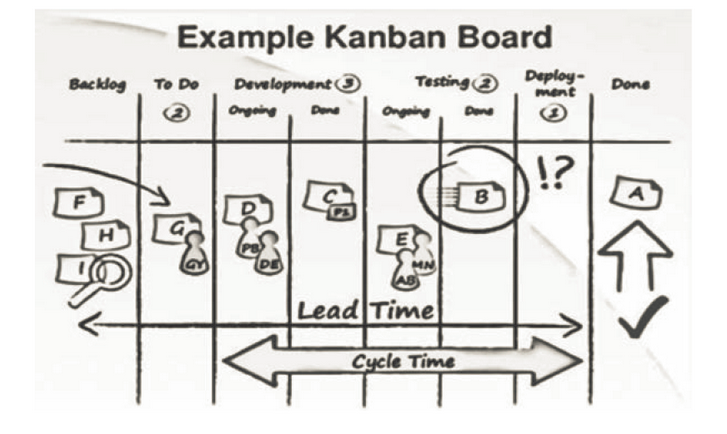
\includegraphics[scale=0.5]{image1.png}
  \caption{Ejemplo de un tablero de Kanban. Extraída de \cite{montegalianoImplantarScrumCon2016}}
  \label{fig:x Tablero kanban}
\end{figure}
\par Las tareas son representadas por tarjetas que avanzan por el tablero a medida que se actualiza su estado actual \cite{montegalianoImplantarScrumCon2016,canosaferreiroSCRUMTeoriaImplementacion2024}. El tablero de trabajo suele tener las siguientes columnas:
\begin{itemize}
    \item \textbf{TO DO}, que representa el trabajo que aún no se ha comenzado.
    \item \textbf{DOING}, que representa el trabajo que se está realizando actualmente.
    \item \textbf{DONE}, que representa el trabajo que se ha completado.
\end{itemize}
\par Este modelo establece una serie de prácticas a seguir:
\begin{itemize}
    \item \textbf{Flujo de trabajo visible}: Las tareas a realizar y el estado en que están son visibles para todos los participantes. Se puede implementar de forma física, utilizando una pared / pizarrón y post-its, o utilizar herramientas como Trello \cite{CaptureOrganizeTackle}. Aún así, es importante plasmar el sistema de forma visual \cite{montegalianoImplantarScrumCon2016,canosaferreiroSCRUMTeoriaImplementacion2024}.
    \item \textbf{Número limitado de tareas}: Para fomentar la agilidad, se limita la cantidad de tareas a realizar. Un miembro del equipo debería tener asignado un número pequeño de tareas en cada columna, de forma que pueda avanzar constantemente. En una situación ideal, un participante es capaz de terminar 1 o 2 tareas al día \cite{montegalianoImplantarScrumCon2016,canosaferreiroSCRUMTeoriaImplementacion2024}.
    \item \textbf{Medir el tiempo de trabajo}: Es importante hacer un seguimiento del avance de las tareas. Recopilar estas métricas permite mejorar los procesos de trabajo y abordar las posibles dificultades que aparezcan  \cite{montegalianoImplantarScrumCon2016,canosaferreiroSCRUMTeoriaImplementacion2024}. Algunas métricas comunes son “lead time”, “touch time” o velocidad, las cuales se estudian en otra sección del trabajo. 
    \item \textbf{Implementar políticas de procesos}: Es necesario establecer criterios que ayuden a mantener un buen ambiente de desarrollo \cite{canosaferreiroSCRUMTeoriaImplementacion2024}. Algunos de ellos pueden ser límite de tareas por personas o protocolos para decidir si una tarea puede ser cancelada o pospuesta. 
\end{itemize}


\section{Métricas}
\par Una forma de observar el progreso de un proyecto es recolectando información sobre las tareas que realizan los developers, y observar si aparecen patrones que indiquen la eficiencia del trabajo realizado. A continuación, se nombran algunas de las métricas comúnmente estudiadas.
%
\subsubsection{Lead Time}
\par Registra el tiempo que toma una tarea, desde que se extrae del Product Backlog hasta que es finalmente entregado. Sirve para estimar tiempos de entrega, medido en días \cite{gaeteEnfoqueAplicacionAgil2021}.
%
\subsubsection{Touch Time}
Registra el tiempo real que toma finalizar una tarea, descontando los posibles periodos de inactividad. Se mide en horas de trabajo \cite{gaeteEnfoqueAplicacionAgil2021}.
%
\subsubsection{Velocidad}
Cantidad de ítems de trabajo completados en cada iteración. Mide la productividad del equipo, y busca maximizar el número de requisitos terminados \cite{gaeteEnfoqueAplicacionAgil2021}.
%
\subsubsection{Requisitos no completados}
Registra la cantidad de requisitos que no se completaron durante la iteración a pesar de haberse establecido como uno \cite{gaeteEnfoqueAplicacionAgil2021}.

% 
% ==== VIDEOJUEGOS ====
%
\chapter{Videojuegos}
\par La industria de los videojuegos es uno de los pilares del entretenimiento actual. A nivel global, en 2024 se esperaba que la industria generara \$USD 187.7 miles de millones en ganancias \cite{buijsmanGlobalGamesMarket2024}. Argentina representa una parte muy pequeña de este mercado, y aún así en 2023 se estimó que el tamaño de la industria fue de \$USD 95.049.600 \cite{delaiglesiaObservatorioIndustriaArgentina2024}.
\bigbreak
\par Más allá de su valor económico, los videojuegos son una industria multidisciplinaria, que nuclea artistas, sonidistas, escritores, y lo más relevante para este trabajo, programadores e ingenieros de software.
\bigbreak
\par Este capítulo describe conceptos básicos de qué es un videojuego, además de adentrarse en la relación entre las metodologías del desarrollo y el desarrollo de uno. Se analizan frameworks utilizados, y sus posibles dificultades. También se habla sobre los ciclos de vida de un juego y el rol general de un ingeniero de software en su creación y gestión.
%
%
\section{Definición de videojuego}
\par Es importante definir qué es un videojuego. Según Scott Rogers \cite{rogersLevelGuiaPara2024}, un juego es una actividad que:
\begin{itemize}
    \item tiene al menos un jugador
    \item tiene reglas
    \item tiene una condición para perder o ganar
\end{itemize}
\par Un videojuego es, entonces, un juego que puede jugarse en una pantalla. Es un software interactivo, orientado principalmente al entretenimiento de las personas. Mediante distintos comandos y controles, se simula una experiencia en la pantalla de un dispositivo \cite{alarconaldanaMetodologiaParaDesarrollo2020}. 
Un videojuego es un producto sumamente complejo ya que fusiona distintos aspectos del arte. Arte visual, sonido, narrativa y otros se utilizan para crear una experiencia interactiva \cite{garciaariasDesarrolloVideojuegosDesde2019}. Esta complejidad se verá reflejada a la hora de elegir una metodología de desarrollo.
\par A lo largo de esta sección, se utilizan palabras comunes al desarrollo del videojuego. Algunas de ellas son:
\begin{itemize}
    \item Mecánica: conjunto de reglas que definen cómo se juega un videojuego. Por ejemplo, en un juego de carreras, la mecánica puede ser que el jugador debe llegar a la meta antes que los demás competidores.
    \item Game designer: persona encargada de diseñar las mecánicas del videojuego. El game designer es responsable de definir cómo se juega, qué se puede hacer, y cómo se interactúa con el videojuego.
    \item Documento de diseño (GDD): documento que define las mecánicas del videojuego. También incluye la historia, los personajes, y otros aspectos relevantes del videojuego.
    \item Assets: un asset es un recurso que se utiliza en el videojuego. Puede ser un modelo 3D, una textura, un sonido, o cualquier otro recurso que se utilice en el videojuego.
    \item Playtesting: proceso en el cual se prueba un videojuego, generalmente por jugadores o testers, con el objetivo de identificar errores, evaluar la jugabilidad y obtener retroalimentación para mejorar la experiencia final de usuario.
\end{itemize} 



\section{Etapas del desarrollo}
\par Mas allá de la metodología elegida por los desarrolladores, los videojuegos suelen pasar por las siguientes fases:
\begin{enumerate}
    \item \textbf{Iniciación}: La iniciación es la fase inicial del desarrollo. En esta, se crea el concepto del videojuego a desarrollar, mediante herramientas como las lluvias de ideas o feedback proveniente en proyectos anteriores \cite{shresthaGameDevelopmentLifecycle2023,widjajaUtilizingGameDevelopment2024,ramadanGameDevelopmentLife2013}.
    \item \textbf{Pre-producción}:  En esta etapa se prueba la idea presentada en la iniciación. Se define el género del juego, las mecánicas e historia que lo conforman, además del aspecto visual y sonoro a seguir. Esta información se plasma en un documento de diseño (GDD). Además, se desarrollan prototipos jugables para probar si la idea es divertida y vale la pena desarrollarla por completo \cite{shresthaGameDevelopmentLifecycle2023,widjajaUtilizingGameDevelopment2024,ramadanGameDevelopmentLife2013}.
    \item \textbf{Producción}: Esta es la etapa más larga y costosa del desarrollo. Consiste en la creación de código y assets que constituyen el juego \cite{shresthaGameDevelopmentLifecycle2023,widjajaUtilizingGameDevelopment2024,ramadanGameDevelopmentLife2013}.
    \item \textbf{Testing}: En esta etapa se realiza una prueba en profundidad de las funcionalidades del juego, con el objetivo de encontrar y arreglar errores.
    \item \textbf{Lanzamiento}:  Una vez el juego está terminado, se lanza al mercado.
    \item \textbf{Post-lanzamiento}: El desarrollo no termina con el lanzamiento, sino que es común continuar actualizando el juego, con parches y nuevo contenido.
\end{enumerate}

\section{GDLC (Ramadan y Widyani)}
\par En una investigación realizada en 2013, Ramadan y Widyani proponen una metodología de trabajo especializada para videojuegos \cite{ramadanGameDevelopmentLife2013}. Para ello, toman las etapas del desarrollo de un prototipo establecidas por Fullerton en su libro “Game Design Workshop: A Playcentric Approach to Creating Innovative Games” \cite{fullertonGameDesignWorkshop2008}. Estas etapas son:
\begin{enumerate}
    \item \textbf{Foundation}: en esta etapa se busca lograr que un prototipo sea divertido. Este prototipo puede consistir de una sola mecánica, y no se preocupa por ser un programa completo, sólo interesa tener un ambiente de testing para verificar que la idea es válida \cite{ramadanGameDevelopmentLife2013,fullertonGameDesignWorkshop2008}. \par Por ejemplo, si se está haciendo un juego de plataformas similar a Super Mario Bros \cite{SuperMarioBros2025}, una mecánica base sería la de saltar. En esta etapa, sería necesario crear un personaje que se eleve en el aire al apretar un botón. El salto debe “sentirse bien”. Esto puede lograrse ajustando el tiempo de respuesta al botón, la altura del mismo, o la velocidad de subida y bajada, entre otros.
    \item \textbf{Structure}: versión refinada del prototipo creado en la etapa anterior. El objetivo es crear suficiente estructura como para que otras personas puedan probarlo. Esto requiere añadir reglas y mecánicas como para que el prototipo pueda ser jugado por alguien que no conoce la visión del juego \cite{ramadanGameDevelopmentLife2013,fullertonGameDesignWorkshop2008}. \par Siguiendo el ejemplo anterior, esta etapa podría consistir en añadir un par de plataformas y pedir a un familiar o amigo que intente subirse a ellas.
    \item \textbf{Formal details}:  en esta etapa se crea una versión completa del prototipo obtenido en la previa. Para ello es necesario asegurarse que la mecánica sea “functional”, “internally complete”, y “balanced” \cite{fullertonGameDesignWorkshop2008}. Estos conceptos se explican más adelante, pero la idea es que la mecánica funciona correctamente (es decir, no tiene bugs) y su uso no tiene una complejidad intermedia. \par Continuando con la idea del salto en un plataformero, esta etapa podría consistir en eliminar errores y asegurarse que el salto funcione correctamente. Algunos temas a resolver podrían ser qué sucede si al saltar el personaje colisiona con la base inferior de la plataforma.
    \item \textbf{Refinement}: las etapas anteriores aseguran que el prototipo sea funcional, pero es posible que parte de la “diversión” se haya perdido en el proceso. Esta etapa revisa este concepto para asegurarse que la mecánica sea lo más cercana a la visión del game designer posible. Es importante testear por accesibilidad, es decir, que la mecánica sea fácil de entender por los jugadores \cite{ramadanGameDevelopmentLife2013,fullertonGameDesignWorkshop2008}. 
\end{enumerate}
\par Cada una de estas etapas está relacionada con uno o varios criterios de calidad. En particular, se utilizan los siguientes criterios:
\begin{itemize}
    \item \textbf{Functional}: indica que la mecánica funciona correctamente \cite{ramadanGameDevelopmentLife2013,fullertonGameDesignWorkshop2008}.
    \item \textbf{Internally complete}: indica si se han abordado todas las posibles reglas de la mecánica \cite{ramadanGameDevelopmentLife2013,fullertonGameDesignWorkshop2008}.
    \item \textbf{Balanced}: indica si la dificultad de la mecánica es correcta, es decir que no es ni muy fácil ni muy difícil \cite{ramadanGameDevelopmentLife2013,fullertonGameDesignWorkshop2008}.
    \item \textbf{Fun}: indica que la mecánica es interesante y entretenida para los jugadores \cite{ramadanGameDevelopmentLife2013,fullertonGameDesignWorkshop2008}.
    \item \textbf{Accessible}: representa que la mecánica es intuitiva y fácil de aprender \cite{ramadanGameDevelopmentLife2013,fullertonGameDesignWorkshop2008}.
\end{itemize}
\par La figura 3.1 muestra las relaciones entre las etapas de un prototipo y los criterios de calidad que busca satisfacer.
%
\begin{figure}[h]
  \centering
  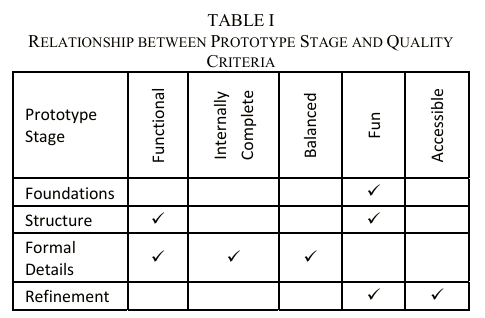
\includegraphics[scale=0.8]{image11.png}
  \caption{Relación entre etapas de prototipo y criterios de calidad. Extraída de \cite{ramadanGameDevelopmentLife2013}.}
  \label{fig:x relacion entre prototipo y criterios de calidad}
\end{figure}
\par Ramadan y Widyani \cite{ramadanGameDevelopmentLife2013} proponen conectar estos conceptos con las etapas del desarrollo de un videojuego. Las fases están siguen un modelo evolutivo, y están compuestas por:
\begin{enumerate}
    \item Initiation: en esta etapa se define la idea general del juego. Se escribe el concepto básico que se formalizará en las siguientes etapas.
    \item Ciclo: en esta fase se crea un documento de diseño y una serie de prototipos, siguiendo los parámetros establecidos por Fullerton \cite{fullertonGameDesignWorkshop2008}.
    \begin{enumerate}
        \item Pre-production: El primer prototipo es “Foundations”, que está relacionado con el criterio de “fun”. A partir de ahí, el resto de prototipos son llamados “Structure”, es decir que cumplen con los criterios de “fun” y “functional” \cite{ramadanGameDevelopmentLife2013}.
        \item Production: en esta etapa se crean los assets y se escribe el código del juego. De este proceso aparecen 2 prototipos 
        \begin{itemize}
            \item “Formal Details”: integra el arte y las mecánicas. Se obtiene un prototipo balanceado, con nuevas features y libre de bugs.
            \item “Refinement”: prototipo completo que busca cumplir con los criterios de “fun” y “accessible”.
        \end{itemize}
        \item Testing: en esta etapa se prueban los prototipos en la etapa anterior. El resultado de esta etapa indica si se pasa a la siguiente fase o si se vuelve a “pre-production”. Ramadan y Widyani \cite{ramadanGameDevelopmentLife2013} nombran 2 métodos de testing:
        \begin{itemize}
            \item Testing de “Formal Details”: se validan la funcionalidad de las mecánicas y la dificultad del juego (cumple con con el criterio “balanced”). Para ello, se realizan sesiones donde los testers juegan el juego y documentan los bugs que encuentren. Además se les pide que documenten cómo se sienten respecto a la dificultad del videojuego.
            \item Testing de “Refinement”: se valida que el prototipo cumple con los criterios de “fun” y “accessibility”. Esto también se realiza con sesiones de juego, pero en este caso se observa el comportamiento del jugador para notar si el prototipo es intuitivo o no.
        \end{itemize}
        \item Beta: en esta fase, se realizan pruebas utilizando testers externos a la empresa. Se utilizan los mismos métodos de la etapa anterior, y también puede resultar en volver a comenzar el ciclo de pre-producción. En caso de encontrar buena recepción, se continúa a la siguiente fase.
    \end{enumerate}
    \item Release: en esta etapa, el proyecto ya está listo para ser lanzado al público.
\end{enumerate}
\begin{figure}[H]
  \centering
  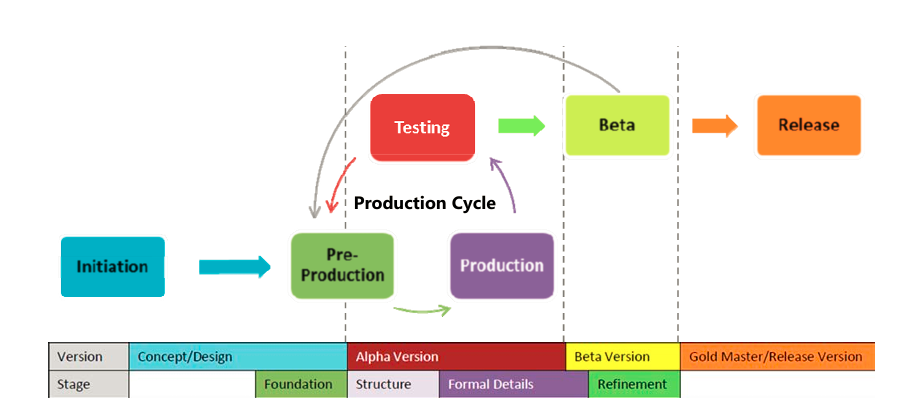
\includegraphics[scale=0.45]{image9.png}
  \caption{El ciclo de desarrollo propuesto por Ramadan y Widyani. Extraída de \cite{ramadanGameDevelopmentLife2013}.}
  \label{fig:x gdlc Ramadan y Widyani}
\end{figure}

\section{Production Point (Anderson)}
\par En su libro, \textit{Production Point} \cite{andersonProductionPointHow2023}, Anderson propone un framework para desarrollar juegos como solo dev. Para ello, separa el proceso en 2 etapas principales:
\begin{itemize}
  \item Pre-production: etapa exploratoria donde se experimentan con sistemas y mecánicas. Se busca la “diversión”, y esto se logra realizando prototipos e iterando sobre ellos. El objetivo es crear un vertical slice.
  \item Production: en esta etapa se crea contenido que apoya a las mecánicas obtenidas  en la preproducción. El objetivo es finalizar el juego.
\end{itemize}
\par Durante \textit{pre-production} (o pre-producción en español), el avance del proyecto sigue una curva exponencial. Esto es porque la integración de mecánicas se dificulta a medida que se añaden nuevas.  Un cambio pequeño puede tener un gran impacto en el juego. Por ejemplo, cambiar la altura del salto en un plataformero 2D puede representar que ciertas plataformas se vuelvan inaccesibles, o que la dificultad de un nivel cambie.
\par En cambio, el progreso durante \textit{production} (producción en español) es lineal. Esto se debe a que el foco es en crear contenido, no mecánicas nuevas. Por ejemplo, crear nuevos niveles debería en promedio tomar el mismo tiempo.
\begin{figure}[H]
  \centering
  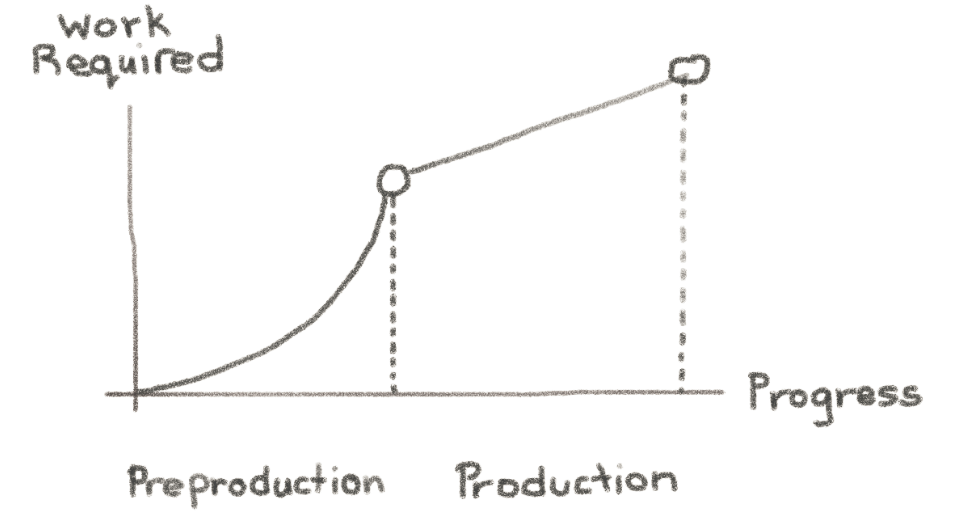
\includegraphics[scale=0.35]{image12.png}
  \caption{Gráfica que representa el progreso en las etapas de \textit{pre-production} y \textit{production}. Extraída de \cite{andersonProductionPointHow2023}.}
  \label{fig:x progreso de etapas Anderson}
\end{figure}
%
%
\subsection{Pre-production}
\par Como se mencionó anteriormente, durante esta etapa se trata de encontrar una mecánica (o varias de ellas) sobre las cuales construir un videojuego. Para ello, durante esta fase se pone un fuerte foco en realizar prototipos. La idea es validar ideas lo más rápido posible, descartando las que no funcionen e iterando sobre las que muestren potencial.
%
\subsubsection{Prototipado}
\par Para validar ideas, Anderson recomienda crear una gran cantidad de prototipos. Idealmente estos prototipos exploran mecánicas distintas, es decir que responden una pregunta de diseño única. Anderson recomienda 2 tipos de prototipado
\begin{itemize}
  \item Prototipos físicos: probar ideas con objetos de la vida real, como papel, juguetes, materiales como madera, etc. El aspecto positivo es que permiten explorar ideas rápidamente, ya que no requieren código o arte. Sin embargo, requieren un fuerte trabajo mental. Para juegos con daño o probabilidad, requiere realizar esos cálculos a mano.
  \item Prototipos digitales: como indica el nombre, son prototipos creados en una computadora. Anderson recomienda no preocuparse por la calidad del código o del arte. El objetivo es probar mecánicas, no crear un software pulido
\end{itemize}
\par Para Anderson, un buen espacio para prototipar son las game jams. En una game jam, los desarrolladores tienen un tiempo limitado para terminar un juego (3 días, 1 semana, etc). Además, suelen presentar al desarrollador con un tema sugerido. Por ejemplo, a finales de enero se realizó la Global Game Jam 2025, donde los participantes tuvieron 3 días para crear un videojuego que cumpliera con el tema “burbujas” \cite{globalgamejamGlobalGameJam2025}.
\bigbreak
\par Anderson también presenta la idea de un juego a la semana. Esta idea se basa en la experiencia de varios desarrolladores:
\begin{itemize}
  \item Bennet Foddy, profesor de game design en la Universidad de Nueva York, enseña una materia donde los alumnos deben crear un juego semanalmente y presentarlo al resto de la clase \cite{GameWeekTeaching}.
  \item “World of Goo” \cite{WorldGooSteam} fue creado en un programa llamado “Experimental Gameplay Project”, llevado a cabo en la Universidad Carnegie Mellon. Este proyecto también duraba una semana, y World of Goo fue uno de los prototipos que los creadores desarrollaron \cite{InterviewGrayGabler,Flashback2008Making}.
  \item Similarmente, “Downwell” \cite{DownwellSteam} fue uno de los prototipos semanales de su creador, Ojiro Fumoto \cite{crecenteHeresOnedev8month2015}. Este proceso fue inspirado por un artículo escrito por otro desarrollador, Rami Ismail, que detalla los beneficios de realizar esta práctica \cite{GameWeekGetting}.
\end{itemize}
\par Durante esta fase, Anderson recomienda validar los prototipos mediante playtesting. El objetivo es obtener feedback abundante y preciso, que permita tomar decisiones informadas sobre una mecánica.
\par Idealmente, se tiene acceso a un grupo grande de personas que puedan probar el juego. Una gran cantidad de información facilita el proceso de entender el feedback recibido. Además, Anderson recomienda grabar las sesiones de playtesting, tanto el gameplay como la cara del tester. La utilidad de esto es poder observar las reacciones inmediatas de los jugadores.
%
\subsubsection{Vertical Slice}
El objetivo de la etapa de pre-producción es crear un vertical slice, es decir, una demo del juego que integra todas las partes de un videojuego. Esto incluye audio, arte, narrativa, interfaz de usuario y mecánicas. Anderson recomienda enfocarse en las siguientes áreas:
\begin{itemize}
  \item Arte y visuales: el aspecto visual de un videojuego es sumamente importante ya que es el primer punto de contacto que los jugadores tienen con un juego. Una buena manera de validar la dirección artística es creando \textit{mockups}\footnote{Mockup: Montaje de distintos elementos artísticos, como arte, sonido, colores, etc.} que incluyan arte, fuentes tipográficas y paletas de color que representen el aspecto visual que se busca. Luego, se puede pedir opiniones a otras personas sobre dicho \textit{mockup}.
  \item Sonido: Similar a las visuales, se pueden crear \textit{mockups} con música y sonidos. Anderson recomienda crear un sistema que permita cambiar los sonidos de objetos en el juego, de forma que se puedan probar rápidamente.
  \item Narrativa: Anderson recomienda utilizar los playtests grabados para validar la narrativa del juego. Con estos videos se puede observar si se está generando la emoción buscada.
  \item Interfaz de usuario: para esta área también se pueden utilizar \textit{mockups}, especialmente de otros juegos que estén en un género similar.
\end{itemize}
%
%
\subsection{Potential Point vs Production Point}
\par La tesis central de Anderson es encontrar el \textit{production point}, es decir, el punto donde pasar de pre-producción a producción. Finalizar la pre-producción no necesariamente significa que se puede avanzar a la siguiente etapa; el vertical slice puede haber tenido malos resultados, con mecánicas confusas y jugadores desinteresados. Anderson llama a este punto \textit{potential point}, e insiste que mover el proyecto a producción en ese momento puede llevar un proyecto al fracaso.
\par Anderson compara 2 prototipos; en el primero, Demonlocke, explica que avanzó a producción teniendo mecánicas sin finalizar, y poco interés por parte del público. En comparación, el segundo proyecto llamado Tic Tac Tanks, comenzó producción con las mecánicas ya definidas, y esta segunda etapa consistió en pulir el juego y añadir contenido.
\begin{figure}[H]
  \centering
  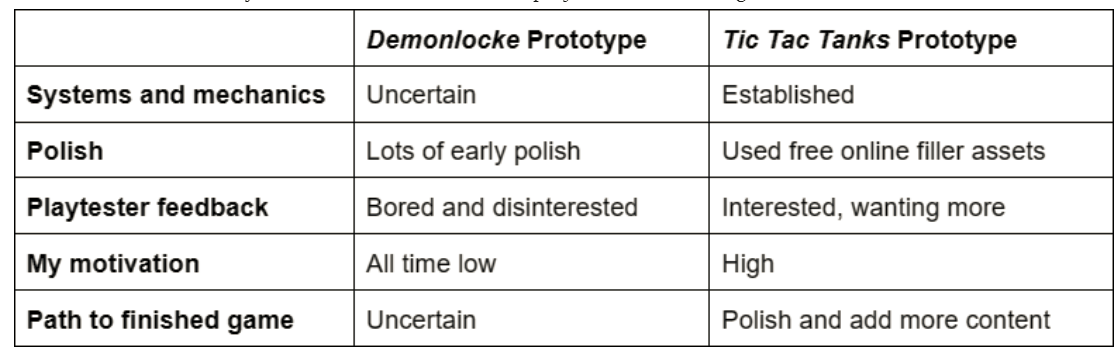
\includegraphics[scale=0.3]{image13.png}
  \caption{Comparación entre Demonlocke y Tic Tac Tanks. Extraída de \cite{andersonProductionPointHow2023}.}
  \label{fig:x Demonlocke vs tic tac tanks}
\end{figure}
\par Anderson propone una serie de preguntas que el proyecto debe contestar para saber en cuál de los puntos se encuentra:
\begin{itemize}
  \item ¿Funcionan todos los sistemas del juego?
  \item ¿Los playtesters disfrutan del juego?
  \item ¿Por cuánto tiempo juegan?
  \item ¿La gente se interesa inmediatamente por este juego a partir de las capturas de pantalla?
  \item ¿Se puede trazar un camino claro para finalizar el proyecto?
\end{itemize}
\par Si se contesta con “no” a alguna de estas preguntas, se recomienda tomar acciones que obtengan una respuesta afirmativa.
%
%
\subsubsection{Production}
\par El objetivo de esta etapa es construir un juego en base a las mecánicas obtenidas en pre-producción. Esto consiste en crear niveles, añadir una historia completa y pulir el arte y sonido. A diferencia de pre-producción, durante esta etapa es imperativo planificar el avance del proyecto y establecer fechas límite. Para ello, Anderson propone 3 acciones:
\begin{itemize}
  \item Establecer un tiempo de juego estimado: definir el largo del juego, generalmente en horas.
  \item Planificar cómo escalar el juego: para llegar a ese tiempo estimado, es importante encontrar formas de aumentar el contenido, lo cual depende del tipo de juego. Por ejemplo, un juego de plataformas tipo Mario Bros puede expandir el juego añadiendo niveles que pongan a prueba distintas habilidades del jugador.
  \item Utilizar herramientas como Kanban para visualizar el avance del proyecto.
\end{itemize}
%
%
\subsection{Alpha y Beta}
El objetivo de esta etapa es pulir el videojuego, de forma que esté preparado para salir al mercado. Algunas de las acciones recomendadas son:
\begin{itemize}
  \item Filtrar el contenido: este proceso se realiza durante la fase de \textbf{alpha} y consiste en eliminar contenido del juego para crear un producto cohesivo. Un buen punto de partida es crear un formulario para quienes prueben el juego, con algunas preguntas como:
    \begin{itemize}
      \item ¿Cuál fue tu pieza de contenido favorita (nivel, personaje, enemigo, etc)?
      \item ¿Cuál fue la pieza de contenido que menos te gustó?
      \item ¿Cuál fue tu acción favorita (habilidad, ataque, etc)?
      \item ¿Cuál fue la acción que menos te gustó?
      \item ¿Si pudieras añadir algo al juego, qué sería?
    \end{itemize}
  \item Corregir bugs: como parte de la \textbf{beta}, se corrigen la mayor cantidad de bugs posible. Requiere tener un grupo grande de testers, que puedan probar el juego en distintas plataformas (Windows, Mac, Linux, Android, IOS, etc). Para mejorar la calidad de los reportes de errores, se recomienda crear un formulario que considere:
    \begin{itemize}
      \item Plataforma o sistema operativo
      \item Especificaciones de hardware
      \item Los pasos para recrear el bug
      \item De ser posible, screenshots o video
      \item Contacto (mail, discord, etc)
    \end{itemize}
  \item Implementar características de calidad de vida (QoL): cambios al juego que mejoran la experiencia de usuario.
  \item Implementar opciones de accesibilidad: esto consiste en opciones como modos de color para personas daltónicas, modificadores de dificultad, etc.
  \item Añadir localización: de ser posible, añadir nuevos idiomas al juego.
\end{itemize}
%
%
\subsection{Launch}
Parte del desarrollo incluye el lanzamiento del juego. Para ello, Anderson recomienda realizar el siguiente proceso:
\begin{enumerate}
  \item Establecer y anunciar la fecha de lanzamiento. Anderson recomienda realizar el anuncio un mes antes de publicar el juego, con el objetivo de formar interés por parte de los jugadores.
  \item Crear un \textit{press kit}. Anderson define un \textit{press kit} como “una colección de texto, imágenes, video del juego y trailers que puede enviarse a la prensa o creadores de contenido \footnote{Creador de contenido: Persona o equipo que crea material audiovisual y lo publica en redes sociales, como Youtube o Twitch.}” \cite{andersonProductionPointHow2023}.
  \item Crear un trailer de lanzamiento, indicando fecha de salida y lugar donde comprar el juego.
  \item Obtener lista de deseados. En plataformas como Steam [47] es imperativo que los potenciales compradores pongan el videojuego en su lista de deseados, ya que les avisará sobre el lanzamiento del mismo. Además, indica a los algoritmos de estas plataformas que hay interés por el juego y esto genera más chances de que sea recomendado a otras personas.
  \item Crear y testear una build \footnote{Build: archivos binarios del juego.} del juego. Muchas plataformas requieren cargar el juego con algunas semanas de anticipación. Este tiempo también es ideal para realizar una última ronda de tests.
  \item Esperar una semana antes de lanzar el juego. Utilizar esta semana para contactar a la prensa y creadores de contenido.
  \item Lanzar el juego.
\end{enumerate}
%
%
\subsection{Post Launch}
\par La última etapa del proceso consiste en revisar las críticas del juego y resolver los bugs que se encuentren. Anderson también menciona la posibilidad de expandir el juego con actualizaciones, sin embargo no entra en detalle de cómo realizar este proceso.
\bigbreak
\par En la figura \ref{fig:x proceso de desarrollo Anderson} se puede observar el proceso completo:
\begin{figure}[H]
  \centering
  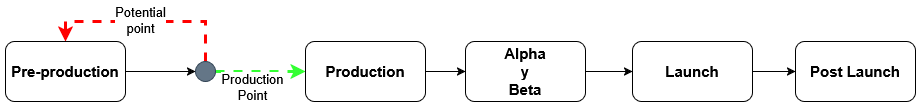
\includegraphics[width=\textwidth]{image8.png}
  \caption{Proceso de desarrollo propuesto por Anderson. Creada por autor.}
  \label{fig:x proceso de desarrollo Anderson}
\end{figure}


\section{Playful Production Process (Lemarchand)}
%
%  -- INTRODUCCION --
%
\par Richard Lemarchand es un game designer prominente en la industria de videojuegos. Trabajó en franquicias populares, como Gex, Soul Reaver y Uncharted \cite{RichardLemarchandcom}. Además, es profesor en la Universidad de Southern California (USC) \cite{RichardLemarchandcom}. En 2021, publicó un libro llamado “A Playful Production Process” \cite{lemarchandPlayfulProductionProcess2021}, donde explora una metodología de desarrollo basada en su experiencia como game designer, productor y profesor. 
\par Para Lemarchand, hay una fuerte conexión entre game design y producción. Es por esto que en su metodología toma conceptos de ambos campos. De forma similar a Ramadan y Widyani, utiliza el libro "Game Design Workshop" \cite{fullertonGameDesignWorkshop2008} como punto de partida.
%
\begin{figure}[H]
  \centering
  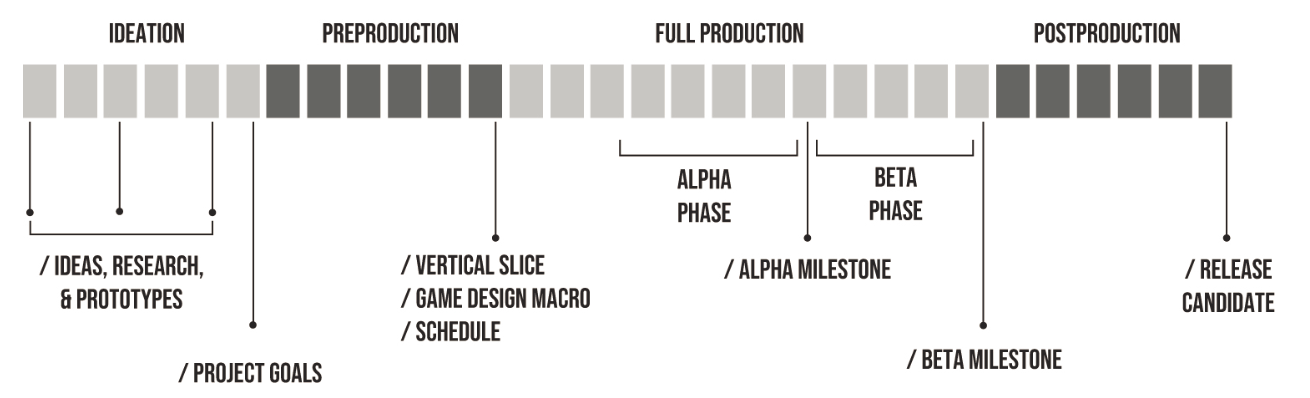
\includegraphics[width=\textwidth]{image6.png}
  \caption{Etapas de la metodología propuesta por Lemarchand. Extraída de \cite{lemarchandPlayfulProductionProcess2021}.}
  \label{fig:x proceso de desarrollo Lemarchand}
\end{figure}
%
%
%  -- IDEATION --
%
\subsection{Ideation}
El proceso de desarrollo comienza en estae etapa, donde se definen una serie de objetivos llamados \textit{player experience goals}. Este concepto es propuesto por Fullerton, que los define como ``una serie de objetivos propuestos por el game designer, que indican el tipo de experiencia que los jugadores tendran durante el videojuego." \cite{fullertonGameDesignWorkshop2008} (Traducción propia).
\par Ejemplos de estos objetivos son ``los jugadores sentirán curiosidad por explorar un universo desconocido.'' o ``los jugadores colaborarán para sobrevivir un mundo post apocalíptico.''. Para establecer estos objetivos, Lemarchand propone una serie de herramientas:
\begin{itemize}
    \item Brainstorming: activadad grupal o individual donde se generan ideas espontáneamente. Lemarchand recomienda enfocarse en la cantidad de ideas, sin preocuparse por su calidad, resaltando la importancia de escribir todas las ideas, incluso las que parecen malas o irrelevantes.
    \item Mind mapping: esta técnica consiste en escribir una idea central y luego conectar ideas relacionadas. 
    \begin{figure}[H]
        \centering
        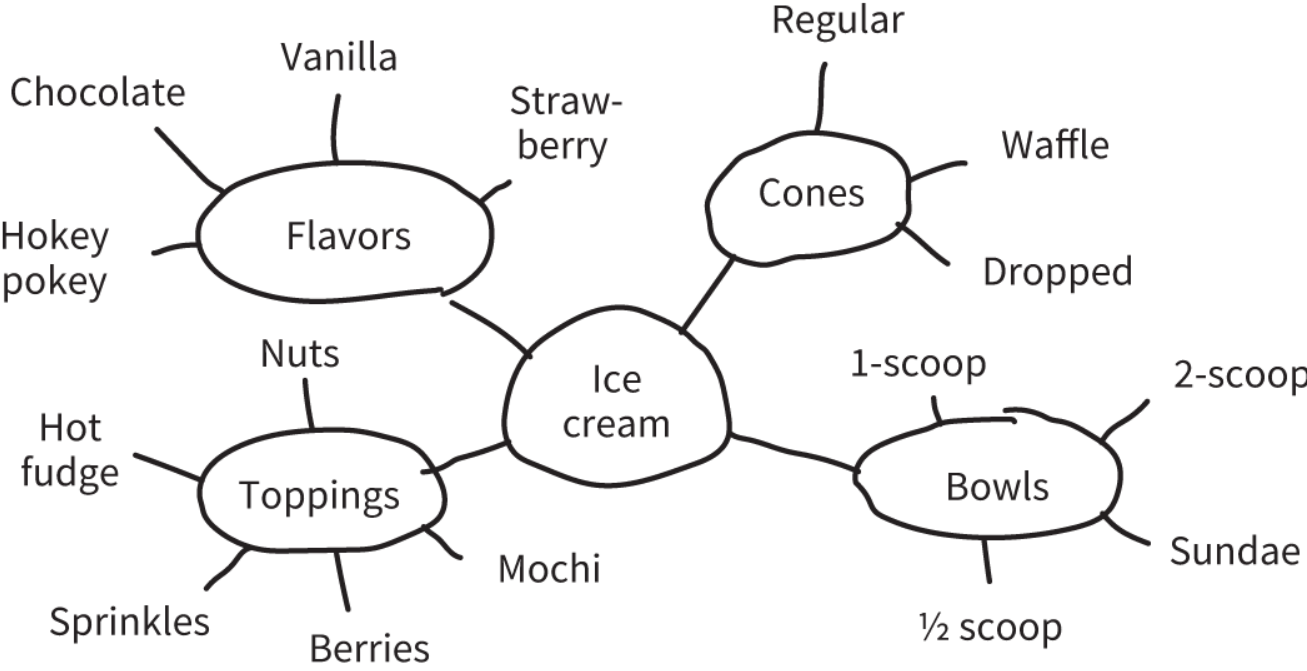
\includegraphics[scale=0.3]{mind_map.png}
        \caption{Ejemplo de un \textit{mind map}. Extraída de \cite{lemarchandPlayfulProductionProcess2021}.}
        \label{fig:x ejemplo de un mind map Lemarchand}
    \end{figure} 
    \item Automastim: este ejercicio consiste en configurar un temporizador y escribir sin parar durante un tiempo determinado. El objetivo es generar ideas espontaneamente, sin preocuparse por la calidad de las mismas.
\end{itemize}
%
%
\subsubsection{Prototipado}
\par Realizar prototipos es una parte fundamental de esta etapa. Lemarchand recomienda empezar con a prototipar lo antes posible, enfocandose en explorar distintas ideas. El objetivo de un prototipo es encontrar un número pequeño de mecánicas (inclusive una sola) que sea interesante o divertida. 
\par Para ayudar en la creación de prototipos, Lemarchand define algunos conceptos de game design. Primero define una \textit{mecánica} como ``reglas y procesos en un juego que lo vuelven funcional e interactivo.''(Traducción propia) \cite{lemarchandPlayfulProductionProcess2021}. Las mecánicas crean acciones llamadas \textit{game verbs}. Algunos ejemplos son saltar, caminar o disparar. Finalmente, define \textit{player activity} como ``el resultado de combinar mecánicas, \textit{game verbs} y narrativa con las acciones del jugador'' (Traducción propia) \cite{lemarchandPlayfulProductionProcess2021}. Por ejemplo, un jugador puede usar la barra espaciadora para ejecutar el \textit{game verb} de saltar. O puede ser un concepto mas abstracto, como tratar de encontrar un final diferente en una historia interactiva.
\par Estos conceptos son importantes porque para Lemarchand, un prototipo debe explorar un \textit{player activity} en particular para decidir si es interesante o no. Para ello, propone una serie de preguntas que un prototipo debe responder:
\begin{itemize}
    \item ¿Qué \textit{player activity} estoy prototipando?
    \item ¿Qué \textit{game verbs} estoy explorando?
    \item ¿Qué emocion evoca este \textit{player activity}?
    \item ¿Qué pregunta o idea se está evaluando con este prototipo?  
\end{itemize}
\bigbreak
\par Similar a Anderson, Lemarchand propone realizar tanto prototipos físicos como digitales. Los prototipos físicos son más rápidos de hacer, pero limitan el tipo de mecánicas que se pueden explorar. Por otro lado, los prototipos digitales son más lentos de hacer, pero permiten explorar una mayor variedad de mecánicas.
\par Playtesting es también una parte importante del proceso. Lemarchand recomienda entregar los prototipos a otras personas lo antes posible, y observar cómo interactuan con ellos. El objetivo es obtener feedback inmediato que informe las próximas iteraciones, notando lo que es interesante y divertido para los jugadores.
%
%
\subsubsection{Project goals}
\par El objetivo final de la etapa de \textit{Ideation} es definir los \textit{project goals}. La idea es que establecer objetivos claros para el proyecto ayuda a guiar el proceso de desarrollo en las siguientes etapas. Lemarchand separa los \textit{project goals} en dos categorias, \textit{experience goals} y \textit{design goals}. 
\bigbreak
\paragraph{Experience goal} Segun Lemarchand, un \textit{experience goal} es ``el tipo de experiencia que se le quiere dar al jugador, generalmente explicada en términos de la experiencia emocional.'' (Traducción propia) \cite{lemarchandPlayfulProductionProcess2021}. Ejemplos de esto puede ser la satisfacción de ganar o el miedo al jugar un juego de terror. La figura \ref{fig:x ejemplo de experience goals Lemarchand} muestra los \textit{experience goals} establecidos para Uncharted, uno de los juegos en los que trabajó el escritor.
%
\begin{figure}[H]
    \centering
    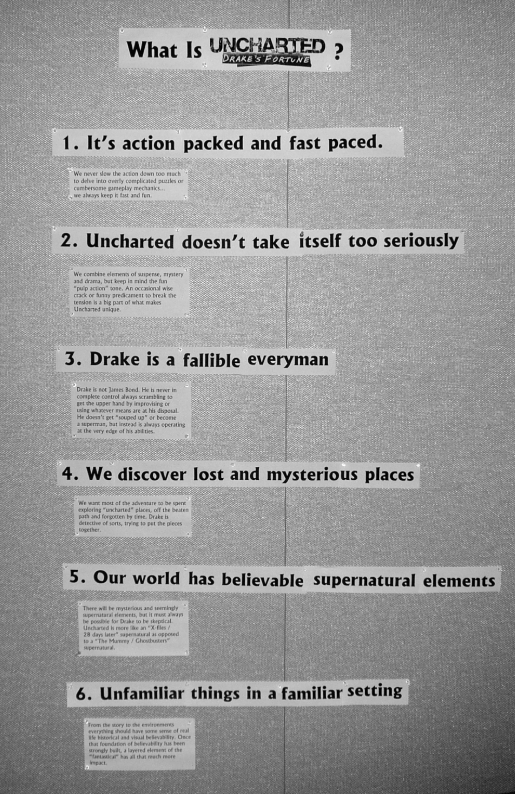
\includegraphics[scale=0.5]{experience_goals.png}
    \caption{``Experience goals'' del videojuego Uncharted. Extraída de \cite{lemarchandPlayfulProductionProcess2021}.}
    \label{fig:x ejemplo de experience goals Lemarchand}
\end{figure} 
%
\paragraph{Design goals} Por otro lado, los \textit{design goals} son las mecánicas que complementan a los \textit{experience goals}. Algunas categorias comunes son:
\begin{itemize}
    \item La plataforma en la que se desarrollará el videojuego (PC, consola, móvil, etc.).
    \item Mecánicas, \textit{game verbs} y \textit{player activities}.
    \item El género del videojuego (plataforma, aventura, rol, etc.).
    \item La dirección artística del videojuego (estilo visual, música, etc.).
\end{itemize}
\par Finalmente, Lemarchand remarca la importancia definir el público objetivo del juego. Para ello, recomienda añadir un \textit{project goal} indicando la audiencia, en el formato ``este juego está dirigido a [audiencia]''.
%
%
%  -- PRE PRODUCTION --
%
\subsection{Pre-production}
\par Lemarchand define a \textit{pre-production}(pre-producción en español) como la etapa donde se se establece el \textit{game design} y el plan a seguir durante la etapa de \textit{production}. Al final de esta etapa, se obtienen 3 artefactos: un \textit{vertical slice}, un \textit{game design macro} y un \textit{schedule}. 
%
%
\subsubsection{Vertical Slice}
Un \textit{vertical slice} es una demo de alta calidad de un videojuego \cite{lemarchandPlayfulProductionProcess2021}. Tanto gráficos, sonido, mecánicas y narrativa deben estar lo suficientemente pulidos como para ser considerados parte del producto final. 
\par Esta demo se construye iterativamente a partir de intentos anteriores, siguiendo un \hyperref[sec:modelos_evolutivos]{modelo evolutivo}. Para ello, se definen una  o varias mecánicas, se crea un prototipo para probarlas, se realiza \textit{playtesting} y se evalúa el resultado. Al final de cada iteración se revisa si el prototipo cumple con los \textit{experience goals} definidos, y si es necesario, se realizan cambios. Este proceso se repite hasta que se obtiene un \textit{vertical slice} que cumple con los objetivos del proyecto.
\begin{figure}[h]
    \centering
    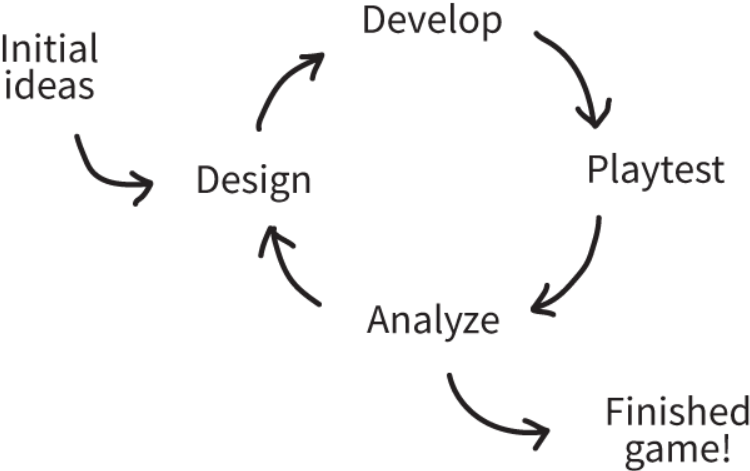
\includegraphics[scale=0.5]{vertical_slice_iteration.png}
    \caption{Proceso iterativo para la creación de un \textit{vertical slice}. Extraída de \cite{lemarchandPlayfulProductionProcess2021}.}
    \label{fig:x iteracion vertical slice}
\end{figure} 
\par Muchos juegos se construyen a partir de un patron repetitivo, llamado \textit{game loop}. Este patrón consiste en una serie de actividades que el jugador puede realizar, como atacar, disparar, saltar, etc. Luego, los \textit{game designers} crean distintas variaciones de estas actividades para mantener el interés del jugador. Este loop se debe ver representado en el \textit{vertical slice}, ya que es una parte fundamental del juego.
%
\par Durante el desarrollo del \textit{vertical slice} es escencial incorporar \textit{playtesting} como una parte fundamental del proceso. Este proceso debe realizarse tanto con otros miembros del equipo como con personas ajenas al proyecto. El objetivo es obtener feedback sobre el \textit{vertical slice} y evaluar si cumple con los \textit{experience goals} definidos. Para ello, Lemarchand propone una serie de prácticas:
\begin{itemize}
    \item \textbf{Minimizar la conversación con el jugador}: esto es útil para observar si el juego es intuitivo y entendible. 
    \item \textbf{Utilizar auriculares}: el sonido es una parte importante de la experiencia de juego, y puede guiar al jugador con el mismo.
    \item \textbf{Escribir los controles del juego en un papel}.
    \item \textbf{Escribir pistas para los problemas que ya se conocen}: es posible que la demo contenga algún bug  que requiera información adicional para que el jugador pueda continuar. En este caso, es recomendable escribir una pista para que el jugador pueda seguir jugando.
    \item \textbf{Sugerir que el jugador piense en voz alta}: el objetivo es obtener más información sobre la experiencia del jugador. Esto puede ayudar a identificar problemas que no son evidentes al observar al jugador.
    \item \textbf{Anotar las acciones del jugador}: escribir lo que el jugador va realizando en un papel puede ayudar a identificar tanto las partes interesantes del juego como las que generan problemas.
    \item \textbf{Realizar entrevistas luego de finalizar}: algunas preguntas recomendadas por Lemarchand son:
    \begin{itemize}
        \item ¿Cuál fue tu momento o interacción favorita?
        \item ¿Cuál fue tu momento o interacción que menos te gustó?
        \item ¿Hubo algo que quisieras hacer y que el juego no te permitiera? 
        \item Si pudieras cambiar algo del juego, ¿qué sería?
    \end{itemize}
\end{itemize}

\par Es importante analizar el feedback obtenido durante este proceso. Para ello, Lemarchand recomienda separar los datos en 3 categorías:
\begin{itemize}
    \item \textbf{Broken/must fix [roto/debe arreglarse]}: estos son problemas de \textit{game design} o bugs que impiden que el jugador tenga la experienca deseada, por lo que deben ser arreglados. Por lo general, la solución suele ser bastante obvia.
    \item \textbf{Question/maybe fix [pregunta/quizás deba arreglarse]}: estos son elementos que quizás no están funcionando correctamente, pero que requiere mayor investigación para determinar el por qué.
    \item \textbf{Suggestion/new idea [sugerencia/nueva idea]}: estas son sugerencias o ideas que pueden mejorar el juego, pero que no son necesarias para que el juego funcione correctamente. Por lo general, estas sugerencias se implementan en iteraciones posteriores.
\end{itemize}
%
%
\subsubsection{Concentric development}
\par Lemarchand propone utilizar \textit{concentric development} durante la etapa de pre-producción, el cual consiste en comenzar por el núcleo del juego y luego ir expandiendo con sistemas que lo complementan. De esta forma, el juego se construye en capas, donde para avanzar a la siguiente capa es necesario que la anterior esté lo suficientemente avanzada como para considerarse parte del producto final. En particular, Lemarchand propone 3 capas:
\begin{itemize}
    \item \textbf{Primary mechanics}: estas son las mecánicas fundamentales del juego. Por ejemplo, en un juego de plataformas, las mecánicas primarias se refiere al movimiento del personaje y de la cámara. A diferencia de la etapa de \textit{Ideation}, estas mecánicas deben ser lo suficientemente pulidas como para ser parte del producto final. Esto significa crear el arte, sonido y programacion y game design necesarios para considerarse completas.
    \item \textbf{Secondary mechanics}: estas mecánicas consisten en los \textit{game verbs} mas importantes del juego, generalmente aquellos que completan el \textit{game loop}. Por ejemplo, en un juego de plataformas, las mecánicas secundarias pueden saltar sobre enemigos o recoger objetos.
    \item \textbf{Tertiary mechanics}: estas mecánicas son las que complementan a las primarias y secundarias. Siguiendo el ejemplo del juego de plataformas, las mecánicas terciarias pueden ser las que permiten al jugador interactuar con el entorno, como abrir puertas o activar interruptores.
\end{itemize}
\par La ventaja de trabajar de esta forma es que al final de pre-producción, se obtiene un \textit{vertical slice} que contiene las mecánicas fundamentales del juego, y estas mecánicas estan lo suficientemente pulidas como para decidir si el proyecto debe continuar o no. 
%
%
\subsubsection{Game Design Macro}
\par Lemarchand define un \textit{game design macro} como ``una matriz de ideas que representa un overview del diseño del juego.'' (Traducción propia) \cite{lemarchandPlayfulProductionProcess2021}. Esta matriz enumera los aspectos más importantes del juego, sin enfocarse en los detalles. Por ejemplo, puede incluir el número de niveles o de personajes. Este artefacto es también una extensión de los \textit{project goals} definidos en la etapa de \textit{Ideation}. El \textit{game design macro} está compuesto de 2 partes: un documento llamado \textit{game design overview} y una tabla llamada \textit{macro chart}.
%
\paragraph{Game Design Overview} Este documento es una visión general del proyecto, y contiene una introducción a los elementos más importantes del juego, incluyendo mecánicas, narrativa y dirección artística. 
%
\paragraph{Macro Chart} Este documento fue originalmente ideado por el desarrollador Mark Cerny, quien lo describe como ``qué tipo de gameplay va en cada lugar'' (Traducción propia) \cite{academyofinteractivearts&sciencesDICESummit20022012}. La idea es que esta tabla contiene los niveles del juego, las mecánicas que se utilizan en cada uno, y los fragmentos de historia que suceden al jugar esa sección.
%
\begin{figure}[H]
    \centering
    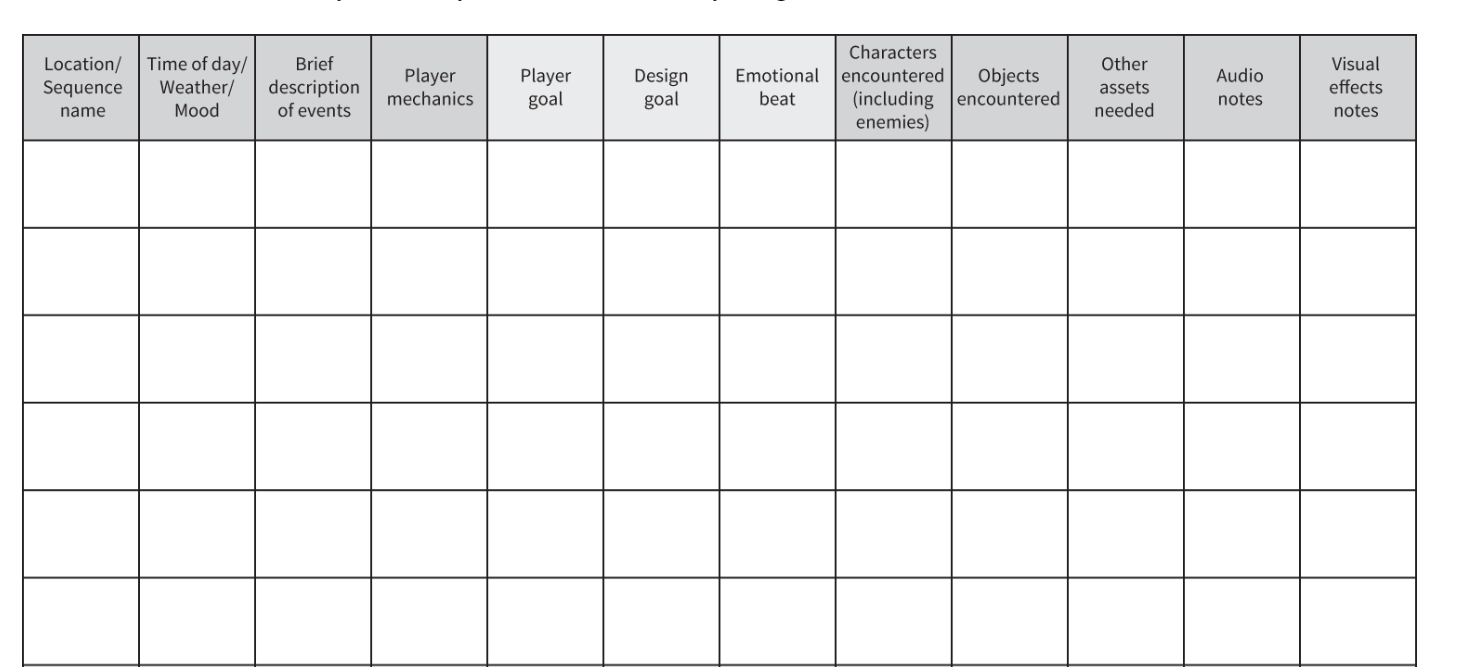
\includegraphics[width=\textwidth]{macro_chart.png}
    \caption{\textit{Macro chart} propuesto por Lemarchand. Extraída de \cite{lemarchandPlayfulProductionProcess2021}.}
    \label{fig:x macro chart}
\end{figure}
%
\par Las columnas \ref{fig:x macro chart} no son definitivas, sino que pueden variar dependiendo del proyecto. Sin embargo, Lemarchand pone énfasis en las siguientes:
\begin{itemize}
    \item \textbf{Player goal}: Lemarchand explica el concepto de \textit{autotelism}(``autolelismo'' en español). Este término, aplicado a videojuegos, se refiere a que cuando una persona juega un juego, establece objetivos para sí mismo basado en lo que el videojuego le permite hacer, lo que quieren hacer, lo que entienden que pueden hacer y lo que han experimentdado de juegos similares \cite{lemarchandPlayfulProductionProcess2021}. En base a esta información, en la columna de \textit{player goal} se debe escribir el objetivo que el jugador debe cumplir en cada sección del juego. Un ejemplo de esto puede ser ``llegar al final del nivel'' o ``derrotar al jefe''.
    \item \textbf{Design goal}: a diferencia del \textit{player goal}, este objetivo está orientado a los \textit{game designers}, y consiste en lo que se desea lograr en términos de mecánicas y narrativa. Por ejemplo, ``introducir la mecánica de saltar'' o ``presentar un nuevo personaje''.
    \item \textbf{Emotional beat}: Esta columna describe lo que se desea que el jugador sienta al jugar esa sección del juego. Por ejemplo, ``sorpresa'' o ``alegría''.
\end 
{itemize}
\par Lemarchand llama \textit{sequences} (secuencias en español) a las filas de la tabla, donde cada una representa una sección del juego. Lemarchand propone una serie de conceptos que ayudan a definir su orden: 
\begin{itemize}
    \item \textbf{Secuenciar gameplay}: para Lemarchand, un buen punto de partida es considerar el orden en que se introducen las mecánicas del juego \cite{lemarchandPlayfulProductionProcess2021}. Por lo general, los \textit{game designers} crean secuencias que añaden mecánicas y dificultad progresivamente.
    \item \textbf{Secuenciar narrativa}: otra herramienta para definir el orden de las secciones es considerar la narrativa del juego. Por ejemplo, es necesario presentar a los personajes, el mundo en el que se desarrolla la historia, y los conflictos que deben resolver. Esto puede ayudar a definir el orden de las secciones del juego.
    \item \textbf{Secuenciar espacio}: otra forma de ordenar las secciones es considerar el espacio en el que suceden, especialmente si el juego está separado en niveles. Lemarchand destaca que crear espacios es una tarea que requiere mucho trabajo, por lo que es importante definir su orden y buscar maneras de reutilizar espacios.
\end{itemize}
\par Por otro lado, es importante considerar la duración de cada secuencia. Por ejemplo, para juegos grandes como \textit{Uncharted}, cada secuencia representa 15 minutos de juego. Para proyectos más pequeños cada sección puede durar entre 1 y 5 minutos. 
\par Finalmente, para completar el \textit{macro chart} se deben añadir el resto de pantallas importantes como el menú principal, el menú de pausa y opciones, y las pantallas de \textit{game over} \footnote{Pantalla que aparece cuando el jugador pierde en el juego.}, de carga y créditos.
%
%
\subsubsection{Schedule}
\par Durante pre-producción, el proceso de desarrollo es iterativo y no sigue un cronograma fijo. En cambio, para la etapa de producción es imperativo programar el progreso de desarrollo mediante un \textit{schedule} (cronograma en español).
\par Para comenzar este proceso, Lemarchand recomienda calcular lo que llama \textit{person-hour}. Este recurso consiste en la cantidad de horas que un miembro del equipo dedica al proyecto. El valor se calcula en base a la cantidad de semanas que se dedicarán al proceso de producción, el número de miembros del equipo y la cantidad de horas que cada uno dedica durante la semana.
\begin{equation}
    T = N \times P \times W
\end{equation}

donde:
\begin{itemize}
    \item $T$ = Total de \textit{person-hours} disponibles para el proyecto.
    \item $N$ = Número de miembros del equipo.
    \item $P$ = Horas-persona que cada miembro trabajará en una semana promedio.
    \item $W$ = Número de semanas dedicadas a producción.
\end{itemize}
\par Por ejmplo, para un equipo de 3 personas, que dedican 20 horas a la semana, durante 10 semanas, el total de \textit{person-hours} disponibles es:
\begin{equation}
    T = 3 \times 20 \times 10 = 600
\end{equation}
\par Luego, este número se compara con el número de \textit{person-hours} que se estima que se necesitan para completar todos los items del \textit{macro chart}, además de otras tareas como participar en reuniones o realizar \textit{playtests}.
\par Lemarchand recomienda comenzar con una tabla que contenga las tareas a realizar en conjunto con las siguientes columnas:
\begin{itemize}
    \item \textbf{Priority (prioridad)}: Esta columna indica la prioridad de cada tarea. Lemarchand propone 3 niveles:
    \begin{itemize}
        \item Priority 1 (prioridad 1): tareas obligatorias, que deben completarse para que el juego funcione correctamente. Por ejemplo, el movimiento del personaje, junto a sus animaciones, controles y sonidos.
        \item Priority 2 (prioridad 2): tareas que son importantes, pero que no son necesarias para que el juego funcione correctamente. Por ejemplo, los \textit{game verbs} utilizados por el jugador para interactuar con el mundo, como ``hablar'' o ``tirar objeto''.
        \item Priority 3 (prioridad 3): tareas que son opcionales, pero que pueden mejorar la experiencia del jugador. Por ejemplo, animaciones adicionales u objetos del entorno de juego.  
    \end{itemize}
    \item \textbf{Hours estimated (horas estimadas)}: Esta columna indica la cantidad de horas que se estima que se necesitan para completar cada tarea. Para Lemarchand, esta columna sólo puede tomar los valores de 1, 2, 4 u 8 horas. Aquellas tareas pequeñas se pueden agrupar en una sola, y las tareas que tomen más de 8 horas deben dividirse en subtareas más pequeñas. El objetivo es reducir la incertidumbre de las estimaciones, y que cada tarea sea lo suficientemente pequeña como para que se pueda estimar con precisión. 
    \item \textbf{Member assigned (miembro asignado)}: Esta columna indica el miembro del equipo que se encargará de cada tarea. Lemarchand recomienda asignar tareas a un solo miembro, ya que esto ayuda a evitar confusiones y conflictos.
\end{itemize} 
%
\begin{figure}[H]
    \centering
    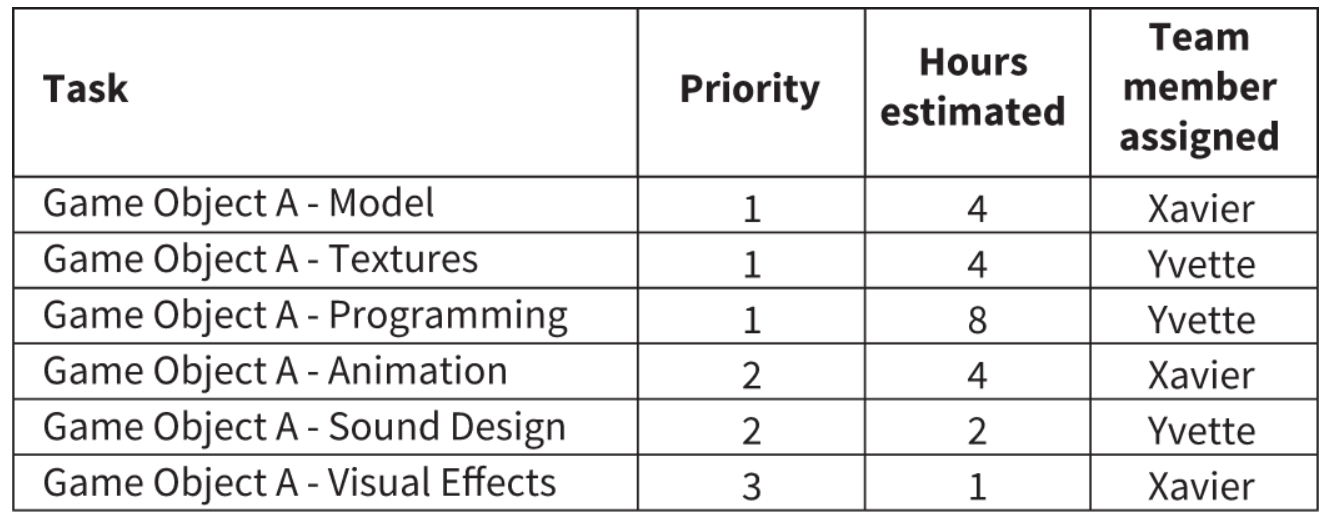
\includegraphics[width=\textwidth]{schedule_example.png}
    \caption{Ejemplo de un \textit{schedule}. Extraída de \cite{lemarchandPlayfulProductionProcess2021}.}
    \label{fig:x schedule ejemplo}
\end{figure}
%
\par Cabe destacar que esta comparación entre \textit{person-hours} disponibles y las horas estimadas para completar las tareas no es una estimación precisa, sino que es una forma de tener una idea general de si el proyecto es viable o no.
\bigbreak
\par Por otro lado, Lemarchand introduce 2 recursos de las metodologías ágiles: los \hyperref[sec:sprint]{sprints} y el \hyperref[sec:burndown_chart]{burndown chart}. Lemarchand separa el trabajo en \textit{sprints} de 2 semanas, y mide su avance mediante el \textit{burndown chart}, utilizando las horas de trabajo estimadas como indicador del progreso.
%
\begin{figure}[H]
    \centering
    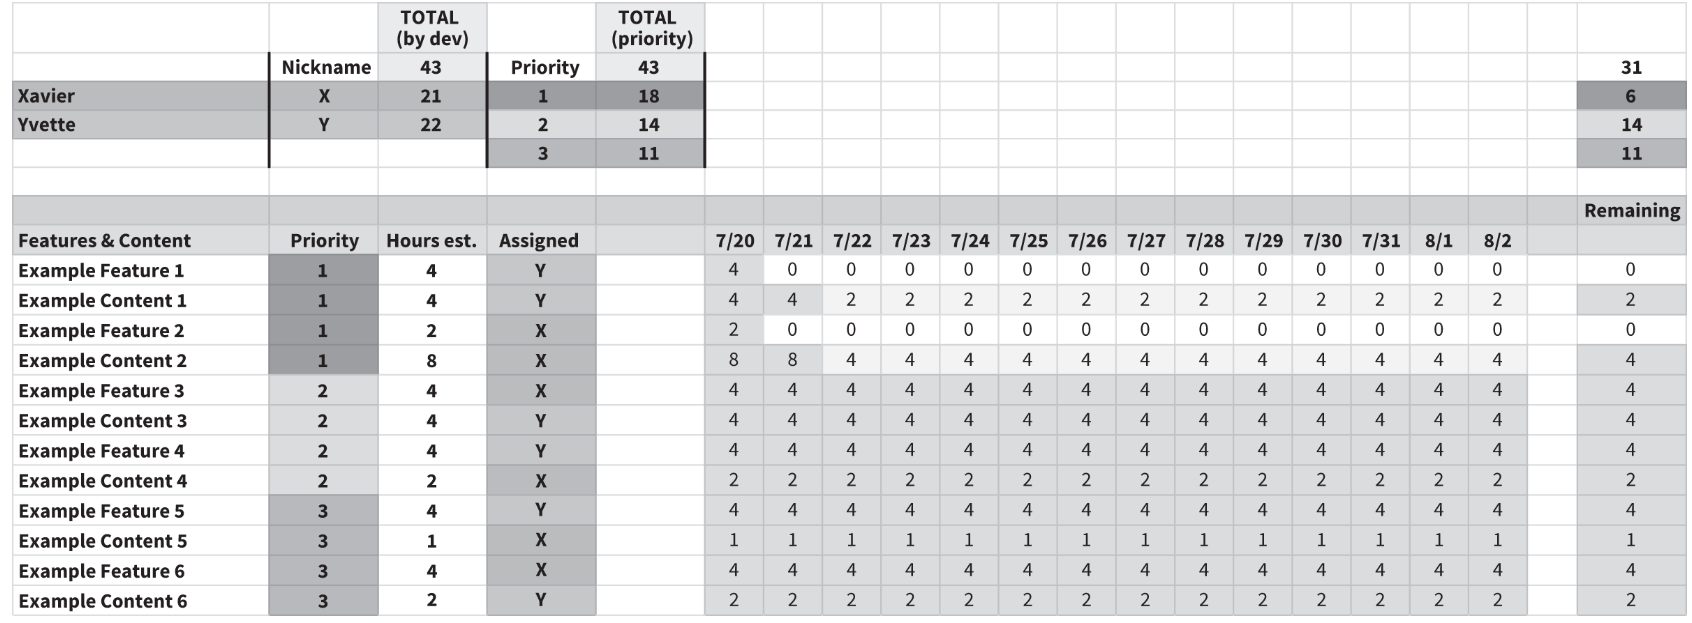
\includegraphics[width=\textwidth]{playful_production_burndown_chart.png}
    \caption{Ejemplo de un \textit{burndown chart} para un \textit{sprint} de 2 semanas. Extraída de \cite{lemarchandPlayfulProductionProcess2021}.}
    \label{fig:x burndown chart Lemarchand}
\end{figure}
%
\subsubsection{Milestone Review}
\par Al final de preproducción, Lemarchand recomienda realizar un \textit{milestone review}. En este evento, el equipo presenta el \textit{vertical slice} tanto a otros desarrolladores como \textit{stakeholders} y líderes del proyecto. El objetivo es obtener feedback sobre el progreso del proyecto y decidir si se debe continuar con la etapa de producción o no. Lemarchand propone una serie de etapas para realizar este evento:
\begin{enumerate}
    \item Los desarrolladores introducen el juego y explican el progreso del proyecto.
    \item Se realiza una demo del juego. Esta demo puede ser jugada por los desarrolladores o por un jugador externo.
    \item El grupo al que se presenta, ya sean \textit{stakeholders} u otros desarrolladores, realizan preguntas y comentarios sobre el juego.
\end{enumerate}
\par Luego de este evento, se debe decidir si el proyecto continúa a la etapa de producción. El proyecto puede no ser aprobado, pero con la posibilidad de realizar cambios y volver a presentar el \textit{vertical slice} en el futuro, o directamente cancelarse para trabajar en un juego distinto.
%
%
%  -- PRODUCTION --
%
\subsection{Production}
\par Si el \textit{vertical slice} es aprobado, el proyecto pasa a la etapa de \textit{production} (producción en español). En esta etapa, se implementan las mecánicas y sistemas definidos en el \textit{game design macro}, y se crea el contenido del juego. Esta etapa tiene 2 hitos principales:
\begin{itemize}
    \item \textbf{Alpha milestone}: en este punto se considera que el juego está en estado \textit{feature complete},es decir que todas las mecánicas y sistemas del juego están implementados, al menos de forma preliminar.
    \item \textbf{Beta milestone}: en este punto se considera que el juego está en estado \textit{content complete}, es decir que todo el contenido del juego está implementado, y sólo faltan ajustes finales y corrección de errores.
\end{itemize}
\par En esta sección se profundiza sobre estos hitos, además de las herramientas que Lemarchand propone para esta etapa.
%
%
\subsubsection{Formal playtesting}
\par Antes de expandir sobre las fases de \textit{Alpha} y \textit{Beta}, Lemarchand introduce el concepto de \textit{formal playtesting}. Comenzando cerca del final de la fase de \textit{Alpha}, Lemarchand propone realizar eventos regulares de \textit{playtesting}, donde se busca obtener datos rigurosos sobre la experiencia del jugador. Este evento se diferencia del \textit{playtesting} informal que se realiza durante la etapa de \textit{Pre-production}, introduciendo una nueva serie de prácticas y herramientas:
\paragraph{Formal Playtest Survey} Se introduce una encuesta que se le entrega al jugador luego de jugar el videojuego. Esta encuesta contiene preguntas sobre la experiencia del jugador, y permite obtener datos cuantitativos y cualitativos sobre el juego. Lemarchand recomienda estructurar las preguntas utilizando la escala Likert, en la cual la respuesta se presenta en una escala gradual, generalmente de 1 a 5, donde 1 representa la respuesta más negativa y 5 la más positiva. La figura \ref{fig:x escala Likert Lemarchand} muestra un ejemplo de este tipo de pregunta, en particular cuestionando si el jugador disfrutó de la calidad de los gráficos del juego.
\begin{figure}[H]
    \centering
    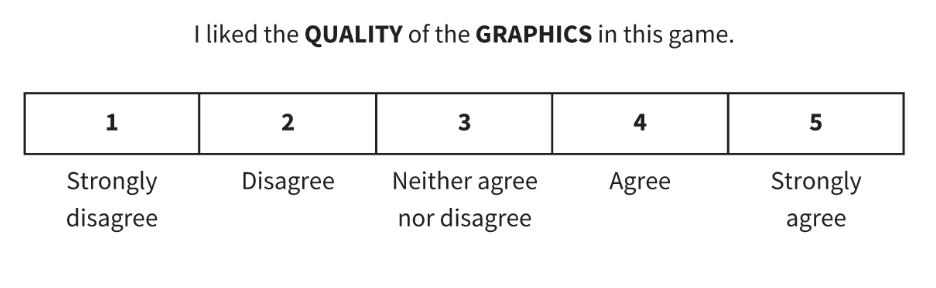
\includegraphics[width=\textwidth]{likert_scale_example.png}
    \caption{Ejemplo de un una pregunta en formato de escala Likert. Extraída de \cite{lemarchandPlayfulProductionProcess2021}.}
    \label{fig:x escala Likert Lemarchand}
\end{figure}
\paragraph{Exit interview} Luego de la encuesta, Lemarchand recomienda realizar una entrevista al jugador, esta vez con preguntas abiertas. Algunas preguntas recomendadas son:
\begin{itemize}
    \item ?`Cómo te hizo sentir x parte del juego?
    \item Describe cómo realizar x acción en el juego.
    \item Describe cómo x sistema funciona. (ej: sistema de inventario)
    \item Describe x personaje. ?`Quién es? ?`Cómo te hizo sentir?
    \item Describe una parte del juego donde te hayas sentido perdido.
\end{itemize}
\paragraph{Game Metrics} Otra herramienta propuesta por Lemarchand es recopilar datos del juego mientras los jugadores realizan el \textit{playtest}. Estos datos pueden incluir el tiempo que el jugador pasa en cada sección del juego así como las distintas acciones que realizan. Esta información pueden ayudar a identificar problemas de diseño y mejorar la experiencia del jugador. Por ejemplo, Lemarchand menciona cómo arreglaron un problema de diseño donde el jugador trataba de utilizar un sistema que permite escalar ciertas estructuras en las zonas incorrectas. Para ello, almacenaron los lugares donde los jugadores saltaban y luego observaban si estos lugares eran los correctos o no.
\begin{figure}[H]
    \centering
    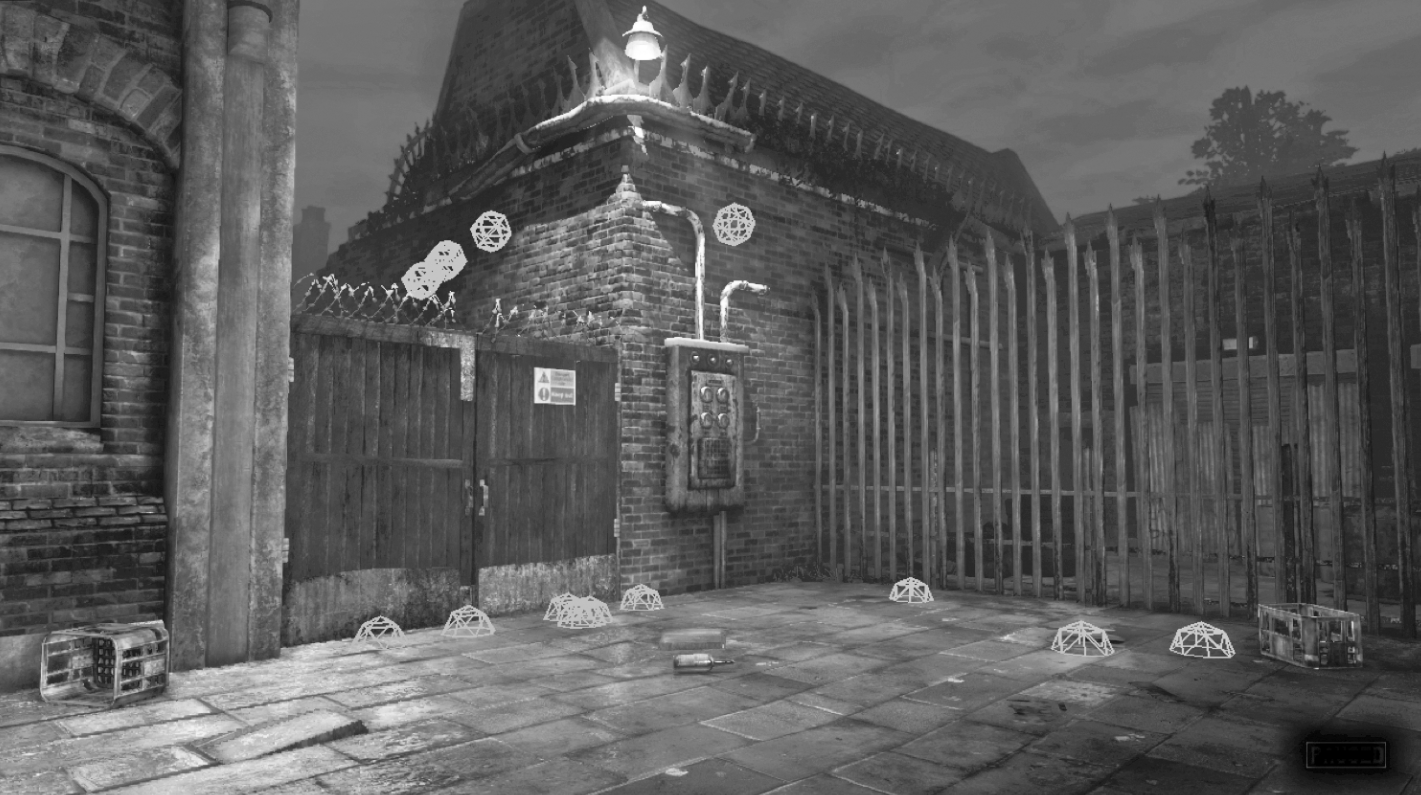
\includegraphics[width=\textwidth]{jump_metrics_example.png}
    \caption{Ejemplo de métricas en el juego \textit{Uncharted}. Las circunferencias indican los lugares donde el jugador realizó saltos. Extraída de \cite{lemarchandPlayfulProductionProcess2021}.}
    \label{fig:x metricas de salto Uncharted Lemarchand}
\end{figure}
%
%
\subsubsection{Alpha Phase}
\par Durante esta fase, los desarrolladores trabajan en completar las mecánicas y sistemas del juego. El objetivo es llegar al \textit{alpha milestone}, donde se considera que el juego esta en estado \textit{feature complete} y \textit{sequence complete}.
\par Lemarchand define una \textit{feature} (funcionalidad en español) como una pieza de funcionalidad dentro del juego \cite{lemarchandPlayfulProductionProcess2021}. Por ejemplo, en un juego de plataformas, una \textit{feature} puede ser el sistema de salto del personaje. Por otro lado, define un \textit{content} (contenido en español) como los \textit{assets} que componene el juego, ya sean sonidos, modelos 3D, texturas, etc. \cite{lemarchandPlayfulProductionProcess2021}. Siguiendo el caso de un juego de plataformas, el contenido puede ser el modelo del personaje, los enemigos y los escenarios. Así, se describen los estados anteriormente mencionados:
\begin{itemize}
    \item \textbf{Feature complete}: Un juego se considera \textit{feature complete} cuando todas las mecánicas y sistemas del juego están implementados, al menos de forma preliminar. Lemarchand recomienda que al menos haya una de cada mecánica en el juego. Por ejemplo, si en el producto final habrá un sistema para hablar con personajes, en la fase de \textit{Alpha} debe haber al menos un personaje y una conversación con el mismo. No es necesario que estén todos los personajes o conversaciones, pero si al menos uno de cada tipo.
    \item \textbf{Sequence Complete} El juego está en estado \textit{sequence complete} cuando todos los niveles están implenentados en el juego, al menos de forma preliminar. El objetivo es que sea posible jugar de principio a fin de forma que se pueda evaluar el ritmo del proyecto \cite{lemarchandPlayfulProductionProcess2021}. Para lograr este estado también se deben implementar los menús como menú principal, de pausa o pantalla de carga.
\end{itemize}
\par Por otro lado, Lemarchand propone diseñar el comienzo del juego en esta etapa. Esta parte del videojuego es muy importante porque es la primera impresión que el jugador tiene del mismo, por lo que debe ser lo suficientemente llamativa e interesante para que quiera seguir jugando. En esta primera parte del juego se deben introducir los controles y las mecánicas principales, además de un gancho narrativo que los mantenga interesados.
\par Además, en esta etapa se comienza el proceso de marketing del producto. Similar a Anderson, Lemarchand recomienda un \textit{press kit} con información sobre el juego, como imagenes y videos, además datos sobre el equipo de desarrollo y el proyecto. Además, recomienda comenzar a publicitar el juego en redes sociales, si embargo no indica herramientas para llevarlo a cabo. Por otro lado, coincide con Anderson en la importancia de contactar con creadores de contenido que tengan una audiencia similar a la del proyecto.
\par Finalmente, durante esta etapa es recomendable implementar un sistema de \textit{bug tracking} (seguimiento de errores en español) que permita registrar errores dentro del juego. En particular, es importante observar:
\begin{itemize}
    \item Errores en los sistemas de juego, como mecánicas que no funcionan correctamente o que no son intuitivas.
    \item Errores en el contenido del juego, como modelos 3D que no se ven bien o texturas que no se cargan correctamente.
    \item Performance del juego, como caídas de frames o tiempos de carga largos.
    \item Problemas de game design, como mecánicas que no son divertidas o que no cumplen con los \textit{experience goals} definidos.
\end{itemize}
\bigbreak
\par Esta etapa concluye con el \textit{alpha milestone}, donde se presenta el progreso del juego tanto a personas ajenas al proyecto como al equipo de desarrollo. El equipo debe presentar la audiencia objetivo, el estado del proyecto (si pueden avanzar a la siguiente etapa o no) y los problemas conocidos del proyecto. En base a esta información, se continúa a la siguiente etapa, la fase de \textit{beta}.
%
%
\subsubsection{Beta Phase}
\par En esta fase se busca llegar al estado \textit{content complete}. Para ello, todas las mecánicas y contenido del juego deben estar implementados lo suficientemente pulido como para ser parte del producto final. Esto incluye:
\begin{itemize}
    \item Todas las mecánicas y sistemas del juego.
    \item Todo el contenido del juego.
    \item Todos los niveles, jugables de principio a fin.
    \item Todos los menús, incluyendo el menú principal, de pausa y de opciones.
    \item El arte para tiendas digitales, incluyendo iconos y material promocional.
\end{itemize}
\par Lemarchand también recomienda accionar sobre los errores de sistemas o diseño que se comenzaron a anotar durante la etapa de \textit{alpha}. No es necesario arreglar todos los errores, pero si aquellos que son más importantes o que afectan la experiencia del jugador.
\bigbreak
\par Esta etapa finaliza en el \textit{beta milestone}. De forma similar al \textit{alpha milestone}, el equipo presenta el progreso del proyecto con el objetivo es obtener feedback sobre el juego y formar un plan con el que continuar a la siguiente etapa. Además, Lemarchand recomienda realizar reuniones internas para discutir las tareas a realizar durante la siguiente fase, \textit{post production} (o post producción en español). 
%
%
%  -- PRODUCTION --
%
\subsection{Post Production}
\par Esta etapa es la última del proceso de desarrollo, y se centra en 3 actividades: \textit{bug fixing} (arreglo de errores), \textit{polishing} (pulido) y \textit{balancing} (balance de diseño). El objetivo es preparar el juego para su lanzamiento, y asegurar que esté en un estado óptimo para los jugadores.
\begin{itemize}
    \item \textbf{Bug fixing}: durante esta etapa se pone un fuerte énfasis en arreglar los errores que se hayan encontrado durante el proceso de producción. El resto de tareas se detienen en favor de esta, y cada cambio se prueba exhaustivamente para asegurarse de que no se introduzcan nuevos errores.
    \item \textbf{Polishing}: esto consiste en realizar pequeños cambios que mejoren la experiencia del jugador. Estos cambios no deben ser grandes, ya que pueden introducir nuevos errores.
    \item \textbf{Balancing}: esta actividad consiste en ajustar las mecánicas del juego para que sean justas y divertidas. Similar al proceso de \textit{polishing}, se recomienda realizar cambios pequeños para evitar nuevos \textit{bugs}.
\end{itemize}
\par En base a estos cambios, se crea un artefacto llamado \textit{release candidate}, el cual se refiere a una \textit{build} del juego que se cree que está lista para ser lanzada. Para ello, el proyecto es tanto \textit{feature complete} como \textit{content complete}, y se han arreglado todos los errores conocidos, además de pasar por un proceso de \textit{polishing} y \textit{balancing}.
\par Finalmente, se realiza un proceso exhaustivo de pruebas para asegurarse que no se encuentra ningun otro error. Si no se encuentran problemas, se obtiene el artefacto \textit{gold master}, el cual es la versión final del juego. 



% 
% ==== BIBLIOGRAFIA ====
%
\printbibliography
\end{document}